% ------------------------------------------------------------------
% Distance by descent: the tower calculus for BB codes — expository draft
% Companion to bb-doubling-theorem.tex (same audience, same notation):
% knows BB construction + group theory + basic ring theory; the doubling
% document is the ideal warm-up but everything needed is re-derived here.
% Build: pdflatex (twice for refs).
% ------------------------------------------------------------------
\documentclass[11pt]{article}

\usepackage[margin=1.05in]{geometry}
\usepackage{amsmath,amssymb,amsthm}
\usepackage{array}
\usepackage{booktabs}
\usepackage{enumitem}
\usepackage{xcolor}
\usepackage{tikz}
\usetikzlibrary{arrows.meta,positioning,shapes.misc,patterns}
\usepackage[most]{tcolorbox}
\usepackage[colorlinks=true,linkcolor=blue!50!black,citecolor=blue!50!black,urlcolor=blue!50!black]{hyperref}

% ---------- theorem environments ----------
\theoremstyle{plain}
\newtheorem{theorem}{Theorem}[section]
\newtheorem{lemma}[theorem]{Lemma}
\newtheorem{proposition}[theorem]{Proposition}
\newtheorem{corollary}[theorem]{Corollary}
\theoremstyle{definition}
\newtheorem{definition}[theorem]{Definition}
\newtheorem{example}[theorem]{Example}
\theoremstyle{remark}
\newtheorem{remark}[theorem]{Remark}

% ---------- boxes ----------
\newtcolorbox{keyidea}[1][]{colback=blue!4!white,colframe=blue!45!black,
  fonttitle=\bfseries,title={#1},breakable,boxrule=0.6pt,left=6pt,right=6pt}
\newtcolorbox{inputbox}[1][]{colback=orange!6!white,colframe=orange!60!black,
  fonttitle=\bfseries,title={#1},breakable,boxrule=0.6pt,left=6pt,right=6pt}
\newtcolorbox{sloganbox}{colback=green!5!white,colframe=green!35!black,
  breakable,boxrule=0.6pt,left=6pt,right=6pt}

% ---------- macros ----------
\newcommand{\F}{\mathbb{F}}
\newcommand{\Z}{\mathbb{Z}}
\newcommand{\suppop}{\operatorname{supp}}
\newcommand{\Ann}{\operatorname{Ann}}
\newcommand{\imD}{\operatorname{im}\Delta}
\newcommand{\Seam}{\operatorname{Seam}}
\newcommand{\clH}{\mathcal{H}}
\newcommand{\base}{\mathrm{base}}
\newcommand{\cov}{\mathrm{cover}}
\newcommand{\Rbase}{\overline{R}}
\newcommand{\Rcov}{R}
\newcommand{\wt}[1]{\lvert #1\rvert}
\newcommand{\ov}[1]{\overline{#1}}

\title{\bfseries Distance by descent: the tower calculus for bivariate
bicycle codes\\[4pt]
\large How the exact distances of published $288$- and $360$-qubit codes
reduce to finite checks at the bottom of a tower of quotients\\[6pt]
\normalsize\normalfont --- expository draft; companion to
\emph{The doubling theorem for bivariate bicycle codes} ---}
\author{}
\date{\today}

\begin{document}
\maketitle

\begin{abstract}
\noindent
The companion document on the \emph{doubling theorem} reads a two-level
tower of bivariate bicycle (BB) codes \emph{upward}: given a small code
with known distance $d$ and four checkable conditions, the doubled code has
distance exactly $2d$. This document reads the same towers \emph{downward},
and drops the conditions. Every BB code whose group has even order sits at
the top of a canonical tower of quotient codes, whether or not any doubling
condition holds; the transport machinery of the doubling proof --- fold,
lift, sheets, the slice identity --- works unconditionally on every rung,
twisted or not; and the doubling theorem's finite \emph{theorem inputs}
(a stabilizer classification, a safe-floor theorem) can be replaced by
finite \emph{certified computations} (censuses with counting certificates,
per-object checks) executed at the bottom of the tower, where the code is
small. The result is a calculus that turns ``what is $d$, exactly?'' for
codes of $300$-plus qubits into minutes of deterministic, auditable
computation with no SAT solver anywhere on the critical path. It resolved
the distance of Bravyi et al.'s $[[360,12,\leq 24]]$ to $d = 24$ --- the
first exact determination of that code's distance --- and reproduced,
solver-free, the two strongest published solver-certified BB distances:
IBM's $[[288,8,20]]$ in ${\sim}105$ seconds and the record
$[[288,12,18]]$ in ${\sim}31$ seconds. Along the way the same machine
re-derives the distance of every intermediate code in each tower, the
censuses it consumes, and a small theory dividend: on \emph{every} free
$\Z_2$ quotient of a BB code, exactly half of the cover's logical classes
are visible downstairs. We develop the calculus from scratch for the same
audience as the companion, prove everything that is provable at a
deliberate pace, flag precisely which finite computations are consumed and
what their certificates contain, and close with the conditions map ---
where the calculus applies, what makes it cheap, and the instances where
it honestly does not reach.
\end{abstract}

\tableofcontents

% ==================================================================
\section{Introduction}
\label{sec:intro}
% ==================================================================

Start from where the companion document ends. The doubling theorem takes a
BB code over $\Z_\ell \times \Z_m$, doubles one cyclic direction, and ---
under four conditions --- concludes that the doubled code's distance is
exactly $2d$. It is a genuine theorem with genuine content, and its
economy is real: every condition lives on the half-size code. But read as
a \emph{method for determining distances}, it has three built-in limits.

\begin{enumerate}[leftmargin=2.2em]
\item \emph{The conditions can fail.} The linchpin condition (R) ---
  equivalently, preservation of the logical count $k$ --- fails on
  documented codes, and when it fails the safe-sector half of the proof
  collapses. The floors can fail even when (R) holds: the companion's
  failure gallery has a code that satisfies the structural conditions and
  still loses distance in its cover.
\item \emph{The inputs are theorems.} The dangerous-sector floor needs a
  \emph{classification} of the base's light stabilizers; the safe-sector
  floor needs a weight theorem about confined classes. For the gross code
  those were proved by hand, at real effort; each new instance re-opens
  the same obligations.
\item \emph{It points upward, one step at a time.} The theorem
  manufactures a bigger code from a smaller one whose distance you must
  already know. It says nothing about a code someone hands you --- and the
  codes people actually hand you are the big ones.
\end{enumerate}

This document is about the inverse reading, developed in the same research
program (\texttt{qec-lab} / \texttt{QECLean}) after the doubling theorem
was in hand. Turn the picture upside down. The published flagship codes
--- gross $[[144,12,12]]$, the record $[[288,12,18]]$, IBM's
$[[288,8,20]]$, Bravyi et al.'s $[[360,12,\leq 24]]$ --- are handed to us
at the \emph{top}. Their groups all have even order, in one or both
directions. Halving an even direction is always possible: it needs no
condition at all, only group theory. So every one of these codes sits at
the top of a canonical \emph{tower} of quotient codes, ending at a code
whose group has odd order in the halved directions --- and the codes at
the bottom are small. The question that drives this document:

\begin{keyidea}[The descent question]
Given a BB code $C$ at the top of its tower of quotients, how much of
$d(C)$ can be \emph{computed} --- not bounded, computed exactly, with
certificates --- from data living at the bottom of the tower?
\end{keyidea}

The answer the program found is: \emph{all of it}, for every instance
within a precisely mapped feasibility envelope --- and the reason is a
structural observation about the doubling proof itself, worth stating up
front because it organizes everything that follows.

\begin{keyidea}[The observation that unlocks descent]
The doubling proof's \emph{architecture} never needed the doubling
theorem's \emph{conditions}. The fold, the diagonal lift, the sector split
by the shadow's class, and the slice identity are unconditional --- they
hold for every free $\Z_2$ quotient of every BB code, even when the cover's
polynomials only descend up to a twist, even when $k$ jumps, even when
(R) fails. What the conditions bought was a specific \emph{answer}
($d = 2d_{\base}$) from finitely many \emph{theorem} inputs. Drop the
demand that the inputs be theorems --- allow finite, certified,
re-checkable computation --- and the architecture itself becomes an
algorithm. Its exponential core (censuses of light objects) migrates down
the tower to the smallest code, and what returns up the tower is a chain
of exact distances.
\end{keyidea}

\paragraph{What it delivered.}
The three headline instances, all closed in the program between
2026-08-10 and 2026-08-11, each end-to-end at \emph{deterministic
certificate} grade with no SAT solver on the critical path
(Section~\ref{sec:engine} defines the grade precisely):

\begin{center}
\small
\begin{tabular}{lllll}
\toprule
code & group & published status & descent result & critical path\\
\midrule
Bravyi et al.\ $[[360,12,\leq 24]]$ & $\Z_{30}{\times}\Z_6$ &
$d \leq 24$ (open) & $d = 24$ \emph{exact} & ${\sim}9.4$ min\\
IBM $[[288,8,20]]$ & $\Z_{18}{\times}\Z_8$ &
$d = 20$ (MILP) & $d = 20$ certified & ${\sim}105$ s\\
record $[[288,12,18]]$ & $\Z_{12}{\times}\Z_{12}$ &
$d = 18$ (solver) & $d = 18$ certified & ${\sim}31$ s\\
\bottomrule
\end{tabular}
\end{center}

The first line is a new value: Bravyi et al.'s Table 3 lists this code
with an upper bound only, and no exact determination existed at any grade;
descent resolved ``$\leq 24$'' to ``$= 24$.'' The other two lines are
solver-free, independently certified reproductions of the two strongest
published solver-exact BB distances --- one of them (the $[[288,12,18]]$
record) a code whose distance floor had resisted the program's own SAT
lanes at every attempt. And the table understates the yield: as a
byproduct, the same sweeps re-derive, solver-free, the exact distance of
\emph{every intermediate code} in each tower --- $[[180,8,12]]$,
$[[90,8,8]]$, $[[144,8,10]]$, $[[72,8,6]]$, $[[72,12,6]]$, $[[36,8,4]]$
--- some of which had previously cost hours of solver time
($3.1$ hours of UNSAT ladders for the $[[180,8,12]]$ floor became $0.04$
seconds).

Three features of the mechanism deserve advance notice, because each is a
theme of the document.

\begin{itemize}[leftmargin=2em]
\item \emph{The costs invert.} Directly certifying ``no logical of weight
  $< 24$'' in a $360$-qubit code was priced at $40$--$60$ hours of
  enumeration ($3.3 \cdot 10^{13}$ nodes) --- and solver UNSAT queries at
  that scale simply die. The tower route runs censuses at $n = 90$
  (seconds), then \emph{lift fibers} --- bounded linear-algebra problems,
  one per censused object --- of which $93$--$97\%$ turn out to be
  infeasible before any search happens. Cheapness is not an accident of
  implementation; Section~\ref{sec:engine} isolates the structural reason.
\item \emph{One machine, every output.} The same census--fiber--rung sweep
  that proves the top-level floor re-derives the middle code's distance,
  the middle code's census, and every sector floor, at every level. The
  tower is not scaffolding erected per theorem; it is a single engine
  whose outputs compose.
\item \emph{Theory falls out.} Making the descent unconditional forced the
  program to re-prove the doubling machinery without (R), and the
  (R)-free versions are sharper: on \emph{every} free $\Z_2$ quotient,
  exactly half the cover's logical classes survive the fold
  (Theorem~\ref{thm:ranklaw}), the number of logical qubits can never grow
  downward (Corollary~\ref{cor:kladder}), and the mysterious confinement
  subspace of the doubling proof is unmasked as the image of the fold on
  classes (Proposition~\ref{prop:seamvsimD}).
\end{itemize}

\paragraph{What we assume, and what we do not.}
The audience is the companion document's: you know the BB construction
(group algebra $\F_2[G]$, two polynomials, two blocks of qubits, CSS check
matrices), basic group theory, and basic ring theory. Having read the
companion helps --- we reuse its notation and cite two of its propositions
--- but this document re-derives everything it needs, at speed over shared
ground and at a deliberate pace over new ground. No homology, no covering
space theory, and no solver literacy are assumed. Where the argument
consumes a finite computation, the computation is flagged in a box, with a
statement of \emph{what was computed}, \emph{what certifies it}, and
\emph{where it lives} in the research repository.

\paragraph{Reading map.}
Section~\ref{sec:frame} fixes notation, recaps the companion's frame in
one page, and introduces the running tower --- the record code
$[[288,12,18]]$ descending through gross to a $36$-qubit code.
Section~\ref{sec:transport} builds the unconditional transport layer:
quotients, decks, twisted lifts, the slice identity, and the carry
equation that controls which base objects lift. Section~\ref{sec:ledger}
proves the class ledger --- the rank law, the two carries, and the
$k$-ladder --- and reconnects it to the doubling theorem's (R).
Section~\ref{sec:trisection} assembles the descent trisection: the
three-way sector split that turns a distance question at the top into
census-plus-rung obligations one level down, recursively.
Section~\ref{sec:engine} describes the three certified computational
species (censuses, lift fibers, rungs) and defines the trust grade.
Sections~\ref{sec:bravyi}--\ref{sec:bb288} run the calculus on the three
headline instances, in increasing order of speed and decreasing order of
detail. Section~\ref{sec:conditions} maps the conditions: what the
calculus needs, what merely helps, what it costs, and where it provably
does not reach. Section~\ref{sec:finding} asks how towers are found and
what else descends ($k$, and the theorems that govern it).
Section~\ref{sec:walls} collects the deficit-wall phenomenology and the
falsified folk-claims --- the program's negative results, which are
load-bearing. Section~\ref{sec:trust} states the trust ladder and the
formal (Lean) status, and Section~\ref{sec:further} points into the
repository.

% ==================================================================
\section{The frame, and the running tower}
\label{sec:frame}
% ==================================================================

\subsection{One page of recap}
\label{sec:recap}

Throughout, $G$ is a finite abelian group $\Z_\ell \times \Z_m$, and
$\F_2[G] = \F_2[x,y]/(x^\ell{=}1,\, y^m{=}1)$ its group algebra; elements
are simultaneously vectors (formal sums of \emph{cells} $x^ay^b$, with
weight $\wt{f}$ the number of cells) and multipliers (acting by ring
multiplication). A BB code over $G$ with polynomials $A, B \in \F_2[G]$
has qubits in two blocks $L \sqcup R$, each indexed by $G$, so
$n = 2\lvert G \rvert$. As in the companion, we work exclusively with
$Z$-type operators $v = (v_L, v_R) \in \F_2[G]^2$; the inversion duality
(companion, \S2.3) transports every statement to the $X$ side, so ``the
distance'' means $d_Z = d_X = d$.\footnote{One bookkeeping note for
readers who go on to the research notes: the notes and scripts run the
mirror ($X$-side) convention. The duality is a weight-preserving bijection
matching cycles to cycles, stabilizers to stabilizers, and censuses to
censuses, so every count quoted in this document is convention-independent.}
The two structure maps are
\[
C(v_L, v_R) := A\,v_L + B\,v_R \in \F_2[G]
\qquad\text{and}\qquad
S(z) := (B\,z,\; A\,z) \in \F_2[G]^2 ,
\]
the \emph{syndrome map} and the \emph{stabilizer map}: $C(v)$ collects the
commutation bits of $v$ against the $X$-checks, and $S(z)$ is the product
of the $Z$-checks at the cells of $z$. A \emph{cycle} is a $v$ with
$C(v) = 0$; a \emph{stabilizer} is an element of $\operatorname{im} S$;
$\operatorname{im} S \subseteq \ker C$ because $C(S(z)) = (AB + BA)z = 0$
--- commutativity of $G$ is the CSS condition. Cycles modulo stabilizers
form the \emph{class space}
\[
\clH := \ker C \,/\, \operatorname{im} S,
\]
a vector space of dimension $k$, the number of logical qubits; the class
of $v$ is $[v]$, and a \emph{nontrivial logical} is a cycle with
$[v] \neq 0$. The distance is
$d = \min\{\wt{v} : v \text{ a cycle},\ [v] \neq 0\}$. Two standard rank
facts get used constantly: $\operatorname{rank} S = \lvert G\rvert - k/2$,
so the \emph{relation space} (the ``metachecks'' of the companion)
\[
K := \ker S = \Ann(A) \cap \Ann(B)
\qquad\text{has}\qquad \dim K = k/2 ,
\]
and by the same count the syndrome map's cokernel $\F_2[G] /
\operatorname{im} C$ also has dimension $k/2$. Both facts follow from the
inversion duality plus rank--nullity; we take them as given.

\subsection{The running tower}
\label{sec:runningtower}

The companion had a running \emph{pair}: gross $[[144,12,12]]$ over its
base $[[72,12,6]]$. This document has a running \emph{tower}, and it is
chosen so that the companion's pair appears inside it as the middle rung:

\begin{center}
\begin{tabular}{llllll}
\toprule
level & group & $A$ & $B$ & parameters & provenance\\
\midrule
$C$ (top) & $\Z_{12} \times \Z_{12}$ & $x^3 + y^2 + y^7$ & $y^3 + x + x^2$
& $[[288,12,18]]$ & the published record\\
gross & $\Z_{12} \times \Z_6$ & $x^3 + y^2 + y$ & $y^3 + x + x^2$ &
$[[144,12,12]]$ & the companion's cover\\
bb72 & $\Z_6 \times \Z_6$ & $x^3 + y + y^2$ & $y^3 + x + x^2$ &
$[[72,12,6]]$ & the companion's base\\
B36 & $\Z_3 \times \Z_6$ & $1 + y + y^2$ & $y^3 + x + x^2$ &
$[[36,8,4]]$ & the bottom\\
\bottomrule
\end{tabular}
\end{center}

Read it downward, because that is the direction everything happens. The
top code is Bravyi et al.'s $[[288,12,18]]$ --- the strongest published
solver-exact BB code. Halve its $y$-direction, reducing $y$-exponents
mod~$6$: the polynomial $A = x^3 + y^2 + y^7$ becomes $x^3 + y^2 + y$,
and $B$ is untouched --- \textbf{and this is the gross code}, exactly, the
hero of the companion document. Halve gross's $x$-direction: the
companion's base bb72. Halve the $x$-direction again, mod~$3$: the term
$x^3$ collapses to $1$, giving a $36$-qubit code, $[[36,8,4]]$, small
enough that \emph{everything} about it can be checked by exhaustive
enumeration ($2^{22}$ cycles, all of them enumerable in seconds).

Three remarks, each previewing a section.

\emph{First}: the three rungs of this tower have three different
characters. On the middle rung (gross over bb72) the cover polynomials are
literally the base polynomials --- the companion's setting, an
\emph{untwisted} lift, and (R) holds there. On the top rung the cover
polynomial $A$ has a term $y^7$ whose exponent exceeds the base range: the
lift is \emph{twisted} (Section~\ref{sec:decks}) --- and (R) still holds.
On the bottom rung the lift is twisted \emph{and} (R) fails: $k$ drops
from $12$ to $8$ on the way down. The calculus will not care about any of
this, which is the point.

\emph{Second}: $k$ reads $12, 12, 12, 8$ down the tower. It never
\emph{increases} downward --- and Section~\ref{sec:ledger} proves that it
never can, on any tower of any BB code.

\emph{Third}: the distances read $18, 12, 6, 4$. Note $18 \neq 2 \cdot
12$: the top rung is \emph{not} a doubling --- the doubling theorem is
silent about this tower even though (R) holds on its top rung, because the
floors fail there (the companion's third failure mode, exhibited by this
very code). Descent is how the program certified $d = 18$ anyway, in
$31$ seconds, in Section~\ref{sec:bb288}. Meanwhile $12 = 2 \cdot 6$: the
middle rung is the doubling theorem's original instance. One tower
carries both behaviors, three rungs apart --- whatever governs the
cover-to-base distance ratio acts \emph{per rung}, not per code, and
Section~\ref{sec:walls} returns to what is known about that ratio.

% ==================================================================
\section{Decks, folds, and transport: the unconditional layer}
\label{sec:transport}
% ==================================================================

This section rebuilds the companion's Section 3 --- fold, swap, diagonal
lift, and their transport identities --- in the generality descent needs:
arbitrary free $\Z_2$ quotients, twisted polynomial lifts, no conditions.
Readers arriving from the companion will recognize every object; the
payoff for re-deriving them is that each proof visibly consumes nothing
about the code, so the machinery applies at every rung of every tower.
New objects appear at the end of the section --- the \emph{carry equation}
and the \emph{lift fiber} --- and they are the ones the engine of
Section~\ref{sec:engine} runs on.

\subsection{Decks and quotients}
\label{sec:decks}

Let $G = \Z_\ell \times \Z_m$ with $m$ even (everything transposes to the
$x$-direction; we write formulas for a $y$-halving to match the running
tower's top rung). The subgroup $\{0, m/2\}$ of the second factor gives a
quotient
\[
\pi : \Z_\ell \times \Z_m \;\to\; \Z_\ell \times \Z_{m/2},
\qquad (a, b) \mapsto (a,\; b \bmod m/2),
\]
with every base cell covered by exactly two cells upstairs: a double
cover, exactly as in the companion but read top-down. Write
$\ov{G} = \Z_\ell \times \Z_{m/2}$, and $\Rcov = \F_2[G]$,
$\Rbase = \F_2[\ov{G}]$ for the two group algebras.

\begin{definition}[deck, fold, sheets]\label{def:deck}
The \emph{deck} of the quotient is the monomial $\sigma := y^{m/2}$: the
unique nonidentity element of $\ker \pi$, acting on $\Rcov$ by
multiplication. The \emph{fold} $p : \Rcov \to \Rbase$ is the ring
homomorphism reducing $y$-exponents mod $m/2$; $p(v)$ is the
\emph{shadow} of $v$. Writing each $y$-exponent uniquely as $b = r + (m/2)s$
with $s \in \{0,1\}$ splits every $v \in \Rcov$ into \emph{sheets}
$v \leftrightarrow (v_0, v_1)$ with $p(v) = v_0 + v_1$, and $\sigma$
swaps the sheets. The \emph{diagonal lift} (or \emph{transfer}) of
$u \in \Rbase$ is
\[
\tau(u) := (u, u) \;=\; (1 + \sigma)\,\widetilde u ,
\]
where $\widetilde u = e_0(u)$ is the copy of $u$ drawn on sheet $0$
(exponents below $m/2$); $e_1(u) := \sigma\, e_0(u)$ is the copy on sheet
$1$. All maps act blockwise on $Z$-operators. Note $\wt{\tau(u)} =
2\wt{u}$, and $\wt{e_i(u)} = \wt{u}$.
\end{definition}

Every order-2 element of $G$ works this way. A rank-two abelian group has
at most three of them --- $x^{\ell/2}$, $y^{m/2}$, and the diagonal
$x^{\ell/2}y^{m/2}$, as parity of $\ell, m$ allows --- so a BB code has at
most three decks, hence at most three quotients, and iterating them builds
the full tower down to the odd part of $G$. Two structural remarks that
came for free in the companion and remain free here: translation by a
nonidentity group element moves \emph{every} cell, so every deck acts
freely (no fixed cells, unlike, say, negation); and $\sigma$ is central
--- multiplication by a ring element commutes with everything in sight ---
which is the one property of $\sigma$ that every proof below actually
uses.\footnote{Central and order 2: for the diagonal deck the sheet split
is by $x$-window and $y$-window jointly; all statements below are proved
via $(1+\sigma)$-algebra and never mention which deck it is. The
non-abelian outlook in Section~\ref{sec:finding} keeps exactly these two
properties and drops commutativity of $G$.}

One typographical inversion, deliberate: the companion decorated the
\emph{cover} with tildes, because there the base was the given object.
Descent inverts the standpoint --- the cover is what you are handed, so it
goes undecorated, and overbars mark the constructed base
($\Rbase$, $\ov A$, $\ov C$, \dots). Sheet-$0$ lifts keep their tildes
($\widetilde u = e_0(u)$).

The master identity and the diagonal lemma port verbatim from the
companion, with the same one-line proofs, and we will use them constantly:
\begin{equation}\label{eq:master}
(1 + \sigma)\, f \;=\; f + \sigma f \;=\; \tau\bigl(p(f)\bigr)
\qquad (f \in \Rcov),
\end{equation}
and for every $f$: $f$ is diagonal ($f_0 = f_1$) $\iff$ $f \in
\operatorname{im}(1+\sigma)$ $\iff$ $(1+\sigma)f = 0$ $\iff$ $p(f) = 0$.
In particular $\ker p = \operatorname{im} \tau$, and $\tau$ is injective.

\subsection{Twisted lifts, and why the calculus never sees them}
\label{sec:twists}

Here is the first genuinely new circumstance. In the companion, base and
cover shared their polynomial expressions, by construction. Descending a
given code, we do not get to choose: the top code's polynomials are what
they are, and their exponents may spill past the base range. On the
running tower's top rung,
\[
A \;=\; x^3 + y^2 + y^7 \quad\text{over } \Z_{12}\times\Z_{12}
\qquad\text{folds to}\qquad
\ov A := p(A) \;=\; x^3 + y^2 + y \quad\text{over } \Z_{12}\times\Z_6 ,
\]
and upstairs $y^7 = y^6 \cdot y = \sigma \cdot y$: the cover polynomial is
the base polynomial's lift \emph{with one term multiplied by the deck}.

\begin{definition}[twisted lift]\label{def:twist}
Fix the fold $p$ and let $\ov A := p(A)$, $\ov B := p(B)$ define the
\emph{base code} of the rung. The rung is an \emph{untwisted} (or
\emph{literal}) lift if $A = e_0(\ov A)$ and $B = e_0(\ov B)$ --- the
companion's setting --- and \emph{twisted} otherwise: some terms of $A$ or
$B$ carry an extra factor $\sigma$ relative to the sheet-$0$ lift.
\end{definition}

Twists look alarming --- they change which cover code sits over a given
base code, and the program's A10 screen showed they genuinely matter for
\emph{constructing} covers (Section~\ref{sec:finding}). The pleasant
surprise, and the reason descent is unconditional, is that for
\emph{transport} they are invisible. Two mechanisms:

\begin{itemize}[leftmargin=2em]
\item \emph{The fold is a ring homomorphism}, so $p(Af) = p(A)\,p(f) =
  \ov A\, p(f)$ --- whatever $A$ is. Twists die under $p$ by definition
  ($p(\sigma) = 1$).
\item \emph{The transfer absorbs twists}: $(1+\sigma)\sigma = \sigma +
  \sigma^2 = 1 + \sigma$, so multiplying by $(1+\sigma)$ cannot tell a
  twisted term from an untwisted one. Precisely: for any $g \in \Rcov$
  with $p(g) = \ov f$, the master identity gives $(1+\sigma)g =
  \tau(\ov f)$ --- \emph{any} lift, twisted or not, has the same
  $(1+\sigma)$-multiple.
\end{itemize}

That is the entire mechanism, and it proves the transport theorem in one
sweep. Write $C, S$ for the cover's maps and $\ov C, \ov S$ for the base's
(built from $\ov A, \ov B$).

\begin{theorem}[deck transport, twist-generic]\label{thm:transport}
For every free $\Z_2$ deck of every BB code, with the base code defined by
the folded polynomials:
\begin{enumerate}[label=\emph{(\arabic*)},leftmargin=2.4em]
\item \emph{Fold is a chain map:} $p \circ C = \ov C \circ p$ and
  $p \circ S = \ov S \circ p$. Hence $p$ maps cycles to cycles and
  stabilizers to stabilizers, and descends to classes:
  $p_* : \clH(\cov) \to \clH(\base)$, $[v] \mapsto [p(v)]$.
\item \emph{Transfer is a chain map:} $C \circ \tau = \tau \circ \ov C$
  and $S \circ \tau = \tau \circ \ov S$. Hence $\tau$ maps cycles to
  cycles and stabilizers to stabilizers, and induces
  $\tau_* : \clH(\base) \to \clH(\cov)$.
\item \emph{Weight:} $\wt{v} \geq \wt{p(v)}$, and $\wt{\tau(u)} = 2\wt{u}$.
\item \emph{Kernel:} $p(v) = 0$ iff $v = \tau(u)$ for some base vector
  $u$; such a $v$ is a cycle iff $u$ is.
\item \emph{Composites:} $p \circ \tau = 0$ and $\tau \circ p =
  (1 + \sigma)$.
\end{enumerate}
\end{theorem}

\begin{proof}
(1) is the ring-homomorphism property applied blockwise, exactly as in the
companion: $p(Av_L + Bv_R) = \ov A\,p(v_L) + \ov B\,p(v_R)$, and
$p(S(z)) = (\ov B\,p(z), \ov A\,p(z)) = \ov S(p(z))$.

(2) is the twist-absorption computation: for a base vector $u$ (per
block), pick the lift $\widetilde u$, so $\tau(u) = (1+\sigma)\widetilde
u$. Then
\[
A\,\tau(u_L) = (1+\sigma)\,A\,\widetilde{u_L}
= \tau\bigl(p(A\,\widetilde{u_L})\bigr) = \tau(\ov A\, u_L),
\]
using centrality of $\sigma$, the master identity~\eqref{eq:master} on the
element $A\widetilde{u_L}$, and (1). Summing blocks gives $C(\tau(u)) =
\tau(\ov C(u))$; the $S$ computation is identical. Note where the twist
went: nowhere --- the computation never wrote $A$ out in terms of $\ov A$.

(3) and (4) are the diagonal lemma, blockwise, as in the companion. (5) is
the master identity again: $p(\tau(u)) = p((1+\sigma)\widetilde u) = 0$
since $p(1+\sigma) = 0$, and $\tau(p(f)) = (1+\sigma)f$.
\end{proof}

\begin{remark}[what just happened]
The companion proved these facts for its one rung and called them ``the
entire compatibility of the two codes.'' The descent-era statement is
stronger in a way that is easy to under-appreciate: \emph{every} BB code
with $2 \mid \lvert G \rvert$ now carries this structure on every deck,
with no hypothesis about how the polynomials interact with the halved
direction. The program validated the theorem numerically on all 22 rungs
of its 11-tower survey --- every chain-map identity, every stabilizer
transport, on twisted and untwisted rungs alike --- not because the proof
is in doubt, but because the \emph{conventions} (which fold, which sheet,
which side) are exactly where implementations err. That falsify-first
habit, theorems re-asserted as executable checks before use, recurs
throughout and is part of why the final certificates deserve trust.
\end{remark}

\subsection{Cycle parity}

One more free-standing lemma, small but consequential. The companion
proved that \emph{stabilizers} have even weight when $\wt A$ and $\wt B$
are odd. The same augmentation argument gives more:

\begin{lemma}[cycle parity]\label{lem:parity}
If $\wt A$ and $\wt B$ are odd, every cycle --- stabilizer or not --- has
even weight. Consequently every distance in sight ($d$ of any code in the
tower, every coset minimum, every censused weight) is even.
\end{lemma}

\begin{proof}
The augmentation $\varepsilon : \F_2[G] \to \F_2$ (evaluate at $x = y =
1$; count terms mod 2) is a ring map with $\varepsilon(A) =
\varepsilon(B) = 1$. If $C(v) = 0$ then $A v_L = B v_R$, so
$\varepsilon(v_L) = \varepsilon(v_R)$ and $\wt{v} = \wt{v_L} + \wt{v_R}
\equiv 2\,\varepsilon(v_L) \equiv 0 \pmod 2$.
\end{proof}

All headline codes have trinomial $A, B$, so the lemma applies to every
tower in this document; it halves every case analysis (odd weights need no
discussion) and will, at one dramatic moment in Section~\ref{sec:bravyi},
delete an entire census obligation with zero computation. The hypothesis
is genuinely load-bearing: the program keeps a $\Z_5 \times \Z_5$ code
with $\wt A = \wt B = 4$ whose covers violate odd-weight conclusions, and
a $(6,6)$ demonstration pair with $\wt A = 4$ owning a weight-7 cycle.
Where $\wt A$ or $\wt B$ is even, the calculus survives with roughly
doubled strata and no parity kills (Section~\ref{sec:conditions}).

\subsection{The slice identity, the carry equation, and lift fibers}
\label{sec:slicecarry}

Now the quantitative heart. Fix a rung and a base vector $b$; which cover
vectors have shadow exactly $b$, and how much do they weigh?

Every cover vector with shadow $b$ can be written --- uniquely, given its
sheet-0 content $v_0 \in \Rbase$ (per block) --- as
\begin{equation}\label{eq:param}
v \;=\; \tau(v_0) + e_1(b),
\qquad\text{sheets } (v_0,\; v_0 + b),
\end{equation}
and the companion's slice identity ports unchanged, with the same
cell-by-cell proof:

\begin{lemma}[slice identity]\label{lem:slice}
For any cover operator $v$ with shadow $b = p(v)$ and sheets
$(v_0, v_0 + b)$:
\[
\wt{v} \;=\; \wt{b} \;+\; 2\,\wt{v_0 \text{ off } \suppop b} .
\]
We call $\wt{v_0 \text{ off } \suppop b}$ the \emph{overflow} of $v$: the
number of base positions outside the shadow's support where the two sheets
are \emph{both} occupied, each such position costing two qubits.
\end{lemma}

So far this is bookkeeping for arbitrary vectors. The question with
content: for which $v_0$ is $v$ a \emph{cycle}? Apply $C$ to the
parametrization~\eqref{eq:param}, using transport
(Theorem~\ref{thm:transport}(2)):
\[
C(v) \;=\; \tau\bigl(\ov C(v_0)\bigr) \;+\; C\bigl(e_1(b)\bigr).
\]
The second term deserves a name. Its shadow is $p(C(e_1 b)) =
\ov C(p(e_1 b)) = \ov C(b)$; so \emph{when $b$ is a base cycle}, the term
$C(e_1(b))$ has zero shadow, hence is diagonal, hence is $\tau$ of a
unique base vector:

\begin{definition}[lift carry]\label{def:liftcarry}
For a base cycle $b$, the \emph{lift carry} $\kappa(b) \in \Rbase$ is the
common sheet of $C(e_1(b))$, i.e.\ $C(e_1(b)) = \tau(\kappa(b))$. It is
computable by two multiplications and a fold, and it does not depend on
which sheet embedding was used ($e_0$ and $e_1$ differ by $\sigma$, which
$\tau$-images absorb).
\end{definition}

Since $\tau$ is injective, the cycle condition for $v$ collapses to a
linear equation \emph{downstairs}:

\begin{theorem}[the carry equation]\label{thm:carry}
Let $b$ be a base vector. Cover cycles with shadow $b$ exist iff $b$ is a
base cycle and the \emph{carry equation}
\[
\ov C(v_0) \;=\; \kappa(b)
\]
is solvable; and then they are exactly $v = \tau(v_0) + e_1(b)$ for $v_0$
in the affine solution set
\[
\mathrm{Fib}(b) \;:=\; v_0^\ast + \ker \ov C
\qquad (\text{any particular solution } v_0^\ast),
\]
a coset of the base's \emph{cycle space}. We call $\mathrm{Fib}(b)$ the
\emph{lift fiber} over $b$.
\end{theorem}

\begin{proof}
If $v$ is a cycle, its shadow $p(v) = b$ is a cycle
(Theorem~\ref{thm:transport}(1)), and $0 = C(v) = \tau(\ov C(v_0) +
\kappa(b))$ forces $\ov C(v_0) = \kappa(b)$ by injectivity of $\tau$.
Conversely, given a cycle $b$ and a solution $v_0$, run the computation
backwards. The solution set of an inhomogeneous linear system is a coset
of the kernel, and $\ker \ov C$ is by definition the base's cycles.
\end{proof}

\begin{keyidea}[Why descent is cheap: read this twice]
Everything the top code can do over a shadow $b$ is now a \emph{linear
algebra problem at the base}: one affine system, base-sized, whose
solution set is a coset of the base's cycle space. Three consequences
power the whole calculus.
\begin{enumerate}[leftmargin=2em]
\item \emph{Solvability is a class condition.} Whether
  $\kappa(b) \in \operatorname{im} \ov C$ depends only on structure; many
  censused shadows simply \emph{have no light lifts at all} --- in
  production, $86$--$97\%$ of fibers are infeasible once the overflow is
  capped (item 3). Emptiness is checked by rank arithmetic, not search.
\item \emph{The fiber is structured.} Its members differ by base cycles,
  so certifying facts about \emph{all} lifts of $b$ means sweeping a coset
  of a space the program already understands one level down --- the same
  species of object as a distance question, ready for recursion.
\item \emph{Weight caps localize the search.} A lift of weight $\leq W$
  has overflow $\leq (W - \wt b)/2$ (slice identity): its sheet $v_0$ may
  act \emph{freely} on $\suppop b$ but touches at most $(W - \wt b)/2$
  cells elsewhere. Enumerating solutions of an affine system that vanish
  almost everywhere off a small window is a bounded, complete,
  certifiable computation (Section~\ref{sec:engine}), and the cap
  $(W - \wt b)/2$ shrinks as the shadow gets heavier --- heavy shadows get
  \emph{cheaper}.
\end{enumerate}
\end{keyidea}

\begin{example}[carries on the companion's rung]\label{ex:carryfamiliar}
On the gross-over-bb72 rung these objects are already familiar from the
companion, under other names. For $b$ a base \emph{stabilizer} $S(z)$, the
fiber contains the stabilizer lifts, e.g.\ sheet-0 contents read off
$\widetilde S(\widetilde z)$ --- the companion computed one explicitly in
its dangerous-sector section (its ``carry'' $c$, supported inside the
shadow's window, is exactly a member of $\mathrm{Fib}(b)$ read on sheet
0). And for $\zeta$ in
the relation space $K$, the companion's \emph{seam carry} $\Delta\zeta$ is
the same mechanism one level up the chain complex: a relation downstairs
breaks upstairs, leaving a diagonal residue. The lift carry $\kappa$ is
the $C$-side twin of the $S$-side $\Delta$, and Section~\ref{sec:ledger}
puts both into one ledger.
\end{example}

\subsection{Two levels: the overflow square}
\label{sec:twolevel}

Towers have several rungs, and the bookkeeping composes. Suppose the base
code itself has a deck, with fold $p'$, shadow $\beta := p'(b)$, and
overflows $m_1$ (top rung, of $v$ over $b$) and $m_2$ (bottom rung, of $b$
over $\beta$). Applying the slice identity twice:

\begin{theorem}[two-level slice]\label{thm:twolevel}
$\wt{v} = \wt{b} + 2m_1 = \wt{\beta} + 2(m_1 + m_2)$, and if $v$ is a
cycle then so are $b$ and $\beta$, with both carry equations in force.
When the two halved directions are \emph{different} axes, the descent
square commutes: folding $x$-then-$y$ or $y$-then-$x$ lands on the same
bottom shadow $\beta$, and the \emph{total} overflow is path-independent
(the \emph{overflow square}), because both totals equal
$(\wt{v} - \wt{\beta})/2$.
\end{theorem}

The overflow square is a pleasing sanity invariant --- the program
verified it on 200 random cycles per mixed-axis tower --- but a curious
empirical footnote is worth recording: across every closed instance,
\emph{no step of any certification ever consumed it}. Mixed-axis towers
(Bravyi-360, the running tower read through its other quotient) and
same-axis towers (IBM-288, where the ``square'' degenerates to a single
descent order) certify identically. Likewise, when both halvings share an
axis the composite is a $\Z_4$ quotient, and one might expect
$\Z_4$-deck theory to be needed: it never was. \textbf{Iterated $\Z_2$
suffices for everything} --- one of the port questions A33 answered by
construction.

% ==================================================================
\section{The class ledger: what half of the code survives the fold}
\label{sec:ledger}
% ==================================================================

The transport layer moves \emph{vectors}. Distance proofs live one level
up, on \emph{classes}: the sector split of Section~\ref{sec:trisection}
sorts a cover logical by the class $[p(v)]$ of its shadow, so before the
calculus can run we must know how the induced maps
\[
p_* : \clH(\cov) \to \clH(\base)
\qquad\text{and}\qquad
\tau_* : \clH(\base) \to \clH(\cov)
\]
behave. In the companion this question was answered under (R), with a
theorem (confinement) whose proof consumed the Bezout certificate. The
descent-era answer is unconditional, sharper, and --- pleasingly ---
almost entirely hand-provable with tools already on the table. This
section proves the ledger; everything in it holds for \emph{every} free
$\Z_2$ deck of \emph{every} BB code, twisted or not, (R) or not.
Throughout, $k := k(\cov)$ and $\ov k := k(\base)$.

\subsection{The pairing, and the adjoint pair}

Two elementary lemmas carry the ledger. The first is the standard CSS
pairing between the two Pauli types, included with proof because its
non-degeneracy is the engine of the rank law.

\begin{lemma}[perfect class pairing]\label{lem:pairing}
For a BB code, the bit-count pairing $\langle v, w\rangle := \sum_q v_q
w_q \in \F_2$ between $Z$-vectors and $X$-vectors descends to a pairing
of a $Z$-class against an $X$-class, and this class pairing is
non-degenerate in both slots.
\end{lemma}

\begin{proof}
An $X$-operator is an $X$-cycle exactly when it commutes with every
$Z$-check, i.e.\ is orthogonal to every row of $H_Z$, i.e.\ lies in
$(\operatorname{im} S)^{\perp}$; symmetrically a $Z$-cycle lies in the
perp of the $X$-stabilizers. So cycles of one type pair to zero against
stabilizers of the other, and the pairing is well defined on classes. For
non-degeneracy, suppose the $Z$-cycle $v$ pairs to zero against
\emph{every} $X$-cycle: then $v \in \bigl((\operatorname{im}
S)^{\perp}\bigr)^{\perp} = \operatorname{im} S$ (double perp over a
finite-dimensional $\F_2$-space), so $[v] = 0$. Symmetrically in the
other slot.
\end{proof}

\begin{lemma}[fold and transfer are adjoint]\label{lem:adjoint}
For every cover $Z$-vector $v$ and base $X$-vector $\ov w$:
$\langle p(v), \ov w\rangle = \langle v, \tau(\ov w)\rangle$.
Consequently, on classes, $p_*$ (on the $Z$ side) and $\tau_*$ (on the
$X$ side) are adjoint with respect to the two class pairings.
\end{lemma}

\begin{proof}
Pure counting, blockwise: at each base cell $q$, the left side adds
$(v_0 + v_1)(q)\,\ov w(q)$ and the right side adds $v_0(q)\,\ov w(q) +
v_1(q)\,\ov w(q)$ --- the two preimage cells of $q$, each carrying a copy
of $\ov w(q)$. As matrices, $\tau$ is literally the transpose of $p$.
Both maps descend to classes by Theorem~\ref{thm:transport} (which holds
verbatim on the $X$ side), and adjointness descends with them.
\end{proof}

\subsection{The rank law}

\begin{theorem}[exactness and the rank law]\label{thm:ranklaw}
For every free $\Z_2$ deck of every BB code:
\begin{enumerate}[label=\emph{(\arabic*)},leftmargin=2.4em]
\item \emph{Exactness at the cover:} $\ker p_* = \operatorname{im}
  \tau_*$ inside $\clH(\cov)$.
\item \emph{The rank law:} $\operatorname{rank} p_* = \operatorname{rank}
  \tau_* = k/2$.
\end{enumerate}
In particular the \emph{seam space}
\[
\Seam \;:=\; \operatorname{im} p_* \;\subseteq\; \clH(\base)
\]
has dimension exactly $k/2$: \textbf{exactly half of the cover's logical
classes survive the fold, and their shadows span a half-$k$-dimensional
subspace of the base's class space} --- however the ranks $k$ and $\ov k$
compare, whatever the twists do.
\end{theorem}

\begin{proof}
(1) One inclusion is $p \circ \tau = 0$. For the other, let $[p(v)] = 0$,
say $p(v) = \ov S(z)$. The corrected vector $v' := v + S(e_0(z))$ is a
cycle in the same class as $v$, and its shadow is $p(v) + \ov S(p(e_0 z))
= \ov S(z) + \ov S(z) = 0$, so $v' = \tau(u)$ with $u$ a base cycle
(Theorem~\ref{thm:transport}(4)), giving $[v] = [v'] = \tau_*[u]$.

(2) Rank--nullity on $\clH(\cov)$ plus (1):
\[
k \;=\; \dim \ker p_* + \operatorname{rank} p_*
\;=\; \operatorname{rank} \tau_* + \operatorname{rank} p_* .
\]
It remains to see the two ranks agree. By Lemma~\ref{lem:adjoint} the
$Z$-side $p_*$ is adjoint to the $X$-side $\tau_*$ across the perfect
pairings of Lemma~\ref{lem:pairing}, and adjoint maps across perfect
pairings have equal rank; the inversion duality (an isomorphism of the
whole picture exchanging the two Pauli types and commuting with $p$ and
$\tau$) then identifies the $X$-side $\tau_*$ with the $Z$-side $\tau_*$
rank-for-rank.
\end{proof}

\begin{remark}[provenance]
The program arrived at this statement the honest way around: measured on
one tower, conjectured, then measured on all 22 rungs of the 11-tower
survey (every rank, every kernel, every image; 22/22), and finally
recognized as a theorem --- the short exact sequence $0 \to \Rbase
\xrightarrow{\tau} \Rcov \xrightarrow{p} \Rbase \to 0$ of chain complexes
has a long exact homology sequence, of which (1) is one joint, and the
adjointness argument supplies the rank symmetry. The proof above is the
same mathematics with the homological algebra unwound by hand, in keeping
with the companion's ground rules. One historical wrinkle: the program's
A33 note briefly attributed ``$\operatorname{rank} \tau_* = k/2$'' to
(R), because it had only ever been measured on (R)-rungs; the A35 survey
refuted the attribution --- the law is universal, and only the
\emph{base}-side halves of the picture belong to (R)
(Section~\ref{sec:Rrevisited}).
\end{remark}

\subsection{The two carries, and the \texorpdfstring{$k$}{k}-ladder}
\label{sec:twocarries}

The rank law fixes the sizes of the four fundamental subspaces; the two
\emph{carry} constructions say who is in them. Both are instances of one
mechanism --- \emph{an identity that holds downstairs breaks upstairs,
and the breakage is diagonal} --- applied to the two structure maps.

\begin{proposition}[lift obstruction; the $C$-side carry]
\label{prop:liftobstruction}
For a base cycle $b$, the following are equivalent:
\emph{(i)} $[b] \in \Seam$;\;
\emph{(ii)} some cover cycle has shadow exactly $b$
(the fiber $\mathrm{Fib}(b)$ of Theorem~\ref{thm:carry} is nonempty);\;
\emph{(iii)} the lift carry satisfies $\kappa(b) \in \operatorname{im}
\ov C$.
Moreover $[b] \mapsto \kappa(b) \bmod \operatorname{im}\ov C$ is a
well-defined linear map $\delta$ on classes, with $\ker \delta = \Seam$;
its rank is $\ov k - k/2$.
\end{proposition}

\begin{proof}
(ii)$\iff$(iii) is Theorem~\ref{thm:carry}. (ii)$\Rightarrow$(i) is the
definition of $p_*$. (i)$\Rightarrow$(ii): if $p(v) = b + \ov S(z)$,
correct as in Theorem~\ref{thm:ranklaw}(1): $v + S(e_0(z))$ is a cycle
with shadow exactly $b$. For well-definedness of $\delta$, change $b$ by
a stabilizer $\ov S(z)$: the cover vector $e_1(\ov S(z)) + S(e_1(z))$ has
zero shadow, hence equals $\tau(w)$ for some $w$; applying $C$ and
transport, $C(e_1 \ov S(z)) = \tau(\ov C(w))$, i.e.\ $\kappa(\ov S(z)) =
\ov C(w) \in \operatorname{im} \ov C$. Linearity is inherited from
$e_1$, $C$, and the sheet-reading; $\ker \delta = \Seam$ restates
(i)$\iff$(iii); and the rank is $\dim \clH(\base) - \dim \Seam = \ov k -
k/2$ by Theorem~\ref{thm:ranklaw}.
\end{proof}

\begin{remark}[the obstruction is generic]\label{rem:obstructiongeneric}
So the liftable classes form a subspace of size $2^{k/2}$ in a class
space of size $2^{\ov k}$: a uniformly random base class lifts with
probability $2^{k/2 - \ov k}$. On the running tower's top rung ($k = \ov
k = 12$) that is $2^{-6}$: of gross's $4096$ classes, only $64$ are
shadows of the record code's cycles. The program measured exactly this
--- 60 out of 60 random gross cycles obstructed, 60 out of 60 true
shadows liftable --- as one of its convention tripwires. For descent the
obstruction is pure profit: fibers over the other $63/64$ of the base are
empty before any enumeration begins.
\end{remark}

The second carry is the companion's: for $\zeta$ in the relation space $K
= \ker \ov S$ (dimension $\ov k/2$; Section~\ref{sec:recap}), the lifted
relation breaks, $S(e_0(\zeta)) = \tau(\Delta\zeta)$, defining the
\emph{seam carry} $\Delta : K \to \clH(\base)$, $\zeta \mapsto
[\Delta\zeta]$. The companion proved --- both directions, without (R),
its lift criterion --- that $\imD$ is exactly the kernel of the transfer
on classes:
\begin{equation}\label{eq:liftcrit}
\ker \tau_* \;=\; \imD .
\end{equation}
(One direction: $\tau(\Delta\zeta) = S(e_0 \zeta)$ is a stabilizer by
construction. The other is the companion's appendix argument, a two-move
normalization; it uses only the diagonal lemma and the master identity,
so it holds verbatim in the twisted setting.) Sizes now come for free,
and with them a structural fact about towers:

\begin{corollary}[the $k$-ladder]\label{cor:kladder}
$\dim \ker \tau_* = \dim \imD = \ov k - k/2$, and consequently
\[
\ov k \;\leq\; k \;\leq\; 2\ov k :
\]
\textbf{descending a deck never increases the number of logical qubits,
and ascending one never more than doubles it.} Both bounds are tight
(gross-over-bb72 has $\ov k = k = 12$; the program's CE1 counterexample
pair has $k = 2\ov k = 24$).
\end{corollary}

\begin{proof}
$\dim \ker \tau_* = \ov k - \operatorname{rank}\tau_* = \ov k - k/2$ by
the rank law; this is $\geq 0$, giving $k \leq 2\ov k$. By
\eqref{eq:liftcrit}, $\ov k - k/2 = \dim \imD \leq \dim K = \ov k / 2$,
giving $\ov k \leq k$.
\end{proof}

Down the running tower, $k$ reads $12, 12, 12, 8$ --- never rising ---
and across the program's full deck survey of the published tables, every
single quotient obeys the ladder; the flagship codes turn out to
\emph{acquire} their $k$ at exactly one rung (where $\ov k < k$) and
carry it unchanged through the rest (Section~\ref{sec:finding}).

\subsection{The Bockstein equality, and the deck-module picture}

One measurement in the ledger is not hand-provable by the tools above,
and the program proved it separately; we state it as a theorem of record
with its provenance, and consume one corollary.

\begin{theorem}[Bockstein equality; program theorems A12--A13,
Lean-backed]\label{thm:bockstein}
For every free $\Z_2$ deck of every BB code (twisted decks included),
\[
\dim\, (1+\sigma)_*\,\clH(\cov) \;=\; k - \ov k
\qquad\text{exactly,}
\]
and as a module over $D := \F_2[\sigma]/(\sigma^2{=}1)$ the cover's class
space decomposes as $\clH(\cov) \cong D^{\,k - \ov k} \oplus
\F_2^{\,2\ov k - k}$. In words: the deck action on classes is as trivial
as the $k$-drop allows, no more and no less --- the number of ``free''
deck-pairs of classes is exactly the number of logical qubits lost on the
way down.
\end{theorem}

The inequality $\geq$ is elementary bookkeeping in the ledger above; the
content is equality, and the program's proof is a small gem worth a
sentence even in an expository sketch: lift the whole situation one more
rung up a $\Z_4$ tower (always possible for group-algebra decks ---
double the same direction again), where the candidate obstruction is
annihilated by a characteristic-2 one-liner; a toy chain complex shows
the statement is \emph{false} for general complexes with deck action, so
the liftability of BB complexes --- ``the next rung always exists'' ---
is the actual content. The theorem is machine-checked
(\texttt{BocksteinLift.lean}, \texttt{BBBocksteinTransport.lean},
axiom-clean) for every doubled-axis cover group with twisted decks
included, and was validated exhaustively on $2^{32}$ polynomial pairs per
deck over the small 2-groups before that.

\begin{corollary}\label{cor:kerinseam}
$\ker \tau_* \subseteq \Seam$, always.
\end{corollary}

\begin{proof}
$(1+\sigma)_* = \tau_* \circ p_*$ on classes (master identity). Its image
is $\tau_*(\Seam)$, of dimension $\dim \Seam - \dim(\Seam \cap \ker
\tau_*) = k/2 - \dim(\Seam \cap \ker\tau_*)$. Setting this equal to $k -
\ov k$ gives $\dim(\Seam \cap \ker \tau_*) = \ov k - k/2 = \dim
\ker\tau_*$.
\end{proof}

\subsection{(R) revisited: the doubling theorem's linchpin, unmasked}
\label{sec:Rrevisited}

The ledger makes short work of the companion's central mystery. Recall
condition (R): \emph{the swap acts trivially on cover classes},
$\sigma_* = \mathrm{id}$.

\begin{theorem}[what (R) really is, descent edition]\label{thm:A12}
For every free $\Z_2$ deck of every BB code, the following are
equivalent:
\emph{(i)} $\sigma_* = \mathrm{id}$ \ (R);\quad
\emph{(ii)} $k = \ov k$;\quad
\emph{(iii)} $1 + \sigma \in (A, B)$ in $\Rcov$ (a Bezout certificate
exists).
\end{theorem}

\begin{proof}
(i)$\iff$(ii): $\sigma_* = \mathrm{id}$ iff $(1+\sigma)_* = 0$ iff $k -
\ov k = 0$, by Theorem~\ref{thm:bockstein}. (iii)$\Rightarrow$(i) is the
companion's Bezout lemma, verbatim: from $PA + QB = 1 + \sigma$, the
element $z := Q v_L + P v_R$ satisfies $S(z) = (1+\sigma)v$ for every
cycle $v$, so $v$ and $\sigma v$ are equivalent.
(ii)$\Rightarrow$(iii) is a counting argument in the quotient ring
(program note A12, elementary): reduction mod $(1+\sigma)$ identifies
$\Rcov/\bigl((1{+}\sigma) + (A,B)\bigr)$ with $\Rbase/(\ov A, \ov B)$,
and $k - \ov k$ measures exactly the failure of $1 + \sigma$ to lie in
$(A,B)$.
\end{proof}

\begin{proposition}[the confined classes, unmasked]\label{prop:seamvsimD}
Under (R), and only under (R),
\[
\Seam \;=\; \ker \tau_* \;=\; \imD :
\]
the seam space coincides with the companion's confined classes. Off (R)
the three cannot all agree --- $\dim \Seam = k/2$ while $\dim \ker\tau_*
= \ov k - k/2$ --- and it is the seam space, not $\imD$, that the safe
sector of descent lives in.
\end{proposition}

\begin{proof}
Under (R), $\ov k = k$, so $\Seam$ and $\ker \tau_*$ both have dimension
$k/2$; Corollary~\ref{cor:kerinseam} gives containment, hence equality;
\eqref{eq:liftcrit} appends $\imD$. Off (R), $\ov k < k$ makes the
dimensions differ.
\end{proof}

\begin{sloganbox}
\textbf{Slogan.} In the doubling proof, ``the safe shadow is confined to
$\imD$'' was a theorem with a certificate. In the descent frame, ``the
safe shadow is confined to $\Seam$'' is a \emph{tautology} --- the shadow
of a class is in the image of the shadow map --- and under (R) the two
statements coincide. What (R) actually buys is not confinement but
\emph{smallness relations}: $k$ preserved, the deck invisible, the seam
computable from base data alone ($\imD$), and --- as
Section~\ref{sec:trisection} will show --- a collapse of the descent
trisection to a single branch. Every one of those is a discount, not a
precondition.
\end{sloganbox}

For calibration, here is the ledger evaluated on the two extreme rungs
the program measured side by side (Bravyi-360's top rung, where (R)
fails, against an (R)-rung of the IBM-288 tower):

\begin{center}
\small
\begin{tabular}{lcc}
\toprule
 & IBM-288 top rung ((R) holds) & Bravyi-360 top rung ((R) fails)\\
\midrule
$(\ov k, k)$ & $(8,8)$ & $(8,12)$\\
$\operatorname{rank} p_* = \operatorname{rank}\tau_* = k/2$ &
$4$ \ \checkmark & $6$ \ \checkmark\\
$\dim \Seam$ & $4$ & $6$\\
$\dim \ker \tau_* = \ov k - k/2$ & $4$ ($= \Seam$) & $2$ ($\subsetneq
\Seam$)\\
$\dim (1+\sigma)_* \clH = k - \ov k$ & $0$ & $4$\\
$\sigma_* = \mathrm{id}$? & yes & no\\
\bottomrule
\end{tabular}
\end{center}

Both columns obey every unconditional row; the (R) column degenerates
exactly where Proposition~\ref{prop:seamvsimD} says it must. The
calculus of the next section consumes only the unconditional rows.

% ==================================================================
\section{The descent trisection}
\label{sec:trisection}
% ==================================================================

We can now assemble the architecture. Fix the top code $C$, one deck with
base $\ov C$, and a \emph{target} $d_t$: the value we intend to certify
as the exact distance ($d_t$ is even wherever cycle parity applies, which
is everywhere in this document). A \emph{violation candidate} is a
nontrivial cover logical $v$ with $\wt v < d_t$, i.e.\ $\wt v \leq W :=
d_t - 2$. The descent trisection sorts every candidate by its shadow, and
hands each branch a finite obligation.

\subsection{The three branches}

\begin{theorem}[descent trisection, one rung]\label{thm:trisection}
Let $v$ be a nontrivial cover logical with $\wt v \leq W$ and shadow $b =
p(v)$. Exactly one of the following holds, with the stated consequences.
\begin{itemize}[leftmargin=2.2em]
\item[\emph{(0)}] \emph{Diagonal branch: $b = 0$.} Then $v = \tau(u)$
  with $u$ a \emph{nontrivial} base logical and $\wt v = 2\wt u \geq
  2\,d(\base)$.
\item[\emph{(i)}] \emph{Dangerous branch: $b \neq 0$, $[b] = 0$.} Then
  $b$ is a nonzero base stabilizer with $\wt b \leq W$, even, and $v$
  lives in $b$'s lift fiber with overflow $m = (\wt v - \wt b)/2 \leq (W
  - \wt b)/2$.
\item[\emph{(ii)}] \emph{Seam branch: $[b] \neq 0$.} Then $[b] \in \Seam
  \setminus 0$ --- at most $2^{k/2} - 1$ classes, however big $\ov k$ is
  --- and $b$ is a weight-$\leq W$ element of one of those classes'
  cosets. Moreover \emph{every} cover cycle over such a $b$ is
  automatically a nontrivial logical, with overflow $\leq (W - \wt
  b)/2$.
\end{itemize}
\end{theorem}

\begin{proof}
(0) If $b = 0$ then $v = \tau(u)$ for a base cycle $u$
(Theorem~\ref{thm:transport}(4)); if $[u] = 0$, say $u = \ov S(z)$, then
$v = \tau(\ov S(z)) = S(\tau(z))$ by transport, contradicting
nontriviality of $v$; so $u$ is a nontrivial logical and $\wt u \geq
d(\base)$.
(i) Stabilizer parity gives $\wt b$ even; the fiber statement is the
slice identity plus Theorem~\ref{thm:carry}.
(ii) $[b] = p_*[v] \in \Seam$ by definition of $p_*$ --- the tautology
advertised above. For automatic nontriviality: any cycle $v'$ over $b$
has $p_*[v'] = [b] \neq 0$, so $[v'] \neq 0$. The weight and overflow
bounds are the slice identity again.
\end{proof}

Each branch converts into an obligation, and the three obligations have
three different characters:

\begin{description}[leftmargin=2em,style=nextline]
\item[(0) needs one number: $d(\base)$.] If $d_t \leq 2\,d(\base)$, the
  diagonal branch is closed by the base's distance --- which descent
  re-derives one level down, recursively, or imports from a prior
  certificate. Note the hard ceiling: \emph{through this branch the
  calculus can never certify more than $2\,d(\base)$ per rung}
  (Section~\ref{sec:conditions}, gate G5). The recursion bottoms out at a
  code small enough to enumerate outright.
\item[(i) needs a census and rungs.] Enumerate, up to translation, every
  nonzero base stabilizer of weight $\leq W$ (\emph{the census});
  for each class, certify that no fiber member of overflow $< M(b) :=
  (d_t - \wt b)/2$ is a nontrivial logical (\emph{the rung}). This is
  precisely the companion's dangerous floor (M), aimed at $d_t$ rather
  than $2d$ --- its census was a classification theorem there (hexagons
  and D-pairs); here it is a certified computation.
\item[(ii) needs coset censuses and per-element rungs.] For each of the
  $\leq 2^{k/2} - 1$ seam classes (translation cuts them to a handful of
  orbits), enumerate every coset element of weight $\leq W$; for each
  \emph{element}, certify that its fiber has no member of overflow $<
  (d_t - \wt b)/2$. By automatic nontriviality these rungs are \emph{pure
  feasibility checks} --- no class dispatch inside the fiber, unlike
  branch (i). This is the doubling template's safe floor, made
  \emph{lift-aware}: the naive hope that every coset element already
  weighs $\geq d_t$ is false in general --- on the IBM-288 tower a
  weight-18 element sits below the target 20; on the running tower the
  seam minima sit at $12 = d(\mathrm{gross})$ against the target 18 ---
  and the per-element fiber check is the repair. Elements whose fibers
  are empty (the vast majority, Remark~\ref{rem:obstructiongeneric} made
  quantitative in Section~\ref{sec:engine}) discharge instantly.
\end{description}

Together with a matching witness, the three obligations assemble into an
exact value; we record the schema once, since all three headline
instances instantiate it verbatim.

\begin{theorem}[assembly schema]\label{thm:assembly}
Suppose, for a target $d_t \leq 2\,d(\base)$:
\emph{(a)} the branch-(i) census is complete to weight $W = d_t - 2$ and
every censused class passes its rung at $M(b)$;
\emph{(b)} the branch-(ii) coset censuses are complete to $W$ and every
censused element passes its per-element rung;
\emph{(c)} some verified cover cycle of weight $d_t$ has nonzero class.
Then $d(C) = d_t$ exactly.
\end{theorem}

\begin{proof}
A violation candidate would fall into a branch of
Theorem~\ref{thm:trisection}: branch (0) contradicts $d_t \leq
2\,d(\base)$; branches (i)/(ii) contradict the rungs via the slice
identity ($\wt v = \wt b + 2m < d_t$ forces $m < M(b)$ over a censused
shadow). So $d(C) \geq d_t$, and (c) caps it. For (c) itself, descent
supplies the class check for free in branch-(ii) style: a witness whose
shadow has nonzero class is nontrivial by transport --- no
$2^{|G|}$-dimensional membership test, the companion's ``subtler than it
looks'' step, is ever run. (The program's witnesses are additionally
re-verified end-to-end from their raw supports on every run.)
\end{proof}

\begin{figure}[ht]
\centering
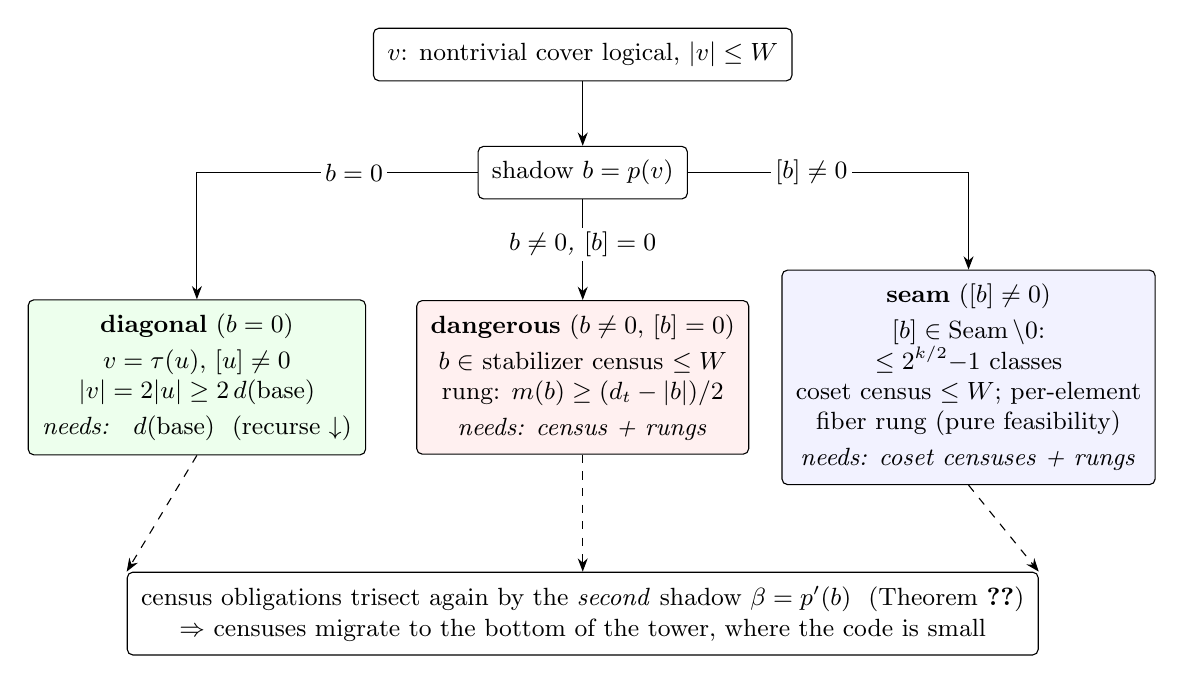
\begin{tikzpicture}[
  box/.style={draw, rounded corners=2pt, align=center, inner sep=5pt,
              font=\small},
  lab/.style={font=\small\itshape, fill=white, inner sep=1.5pt},
  >={Stealth}]
\node[box] (v) at (0,0) {$v$: nontrivial cover logical, $\wt v \leq W$};
\node[box] (q) at (0,-1.5) {shadow $b = p(v)$};
\node[box, fill=green!7] (diag) at (-4.9,-4.1)
  {\textbf{diagonal} ($b = 0$)\\[2pt]
   $v = \tau(u)$, $[u] \neq 0$\\
   $\wt v = 2\wt u \geq 2\,d(\base)$\\[2pt]
   \emph{needs: } $d(\base)$ \ (recurse $\downarrow$)};
\node[box, fill=red!6] (dang) at (0,-4.1)
  {\textbf{dangerous} ($b \neq 0$, $[b]=0$)\\[2pt]
   $b \in$ stabilizer census $\leq W$\\
   rung: $m(b) \geq (d_t - \wt b)/2$\\[2pt]
   \emph{needs: census + rungs}};
\node[box, fill=blue!5] (seam) at (4.9,-4.1)
  {\textbf{seam} ($[b] \neq 0$)\\[2pt]
   $[b] \in \Seam\setminus 0$:\\
   $\leq 2^{k/2}{-}1$ classes\\
   coset census $\leq W$; per-element\\
   fiber rung (pure feasibility)\\[2pt]
   \emph{needs: coset censuses + rungs}};
\node[box] (rec) at (0,-7.1)
  {census obligations trisect again by the \emph{second} shadow
   $\beta = p'(b)$ \ (Theorem~\ref{thm:secondshadow})\\
   $\Rightarrow$ censuses migrate to the bottom of the tower, where the
   code is small};
\draw[->] (v) -- (q);
\draw[->] (q.west) -| node[lab, pos=0.22]{$b=0$} (diag.north);
\draw[->] (q) -- node[lab, pos=0.45]{$b \neq 0$, $[b]=0$} (dang);
\draw[->] (q.east) -| node[lab, pos=0.22]{$[b]\neq 0$} (seam.north);
\draw[->, dashed] (dang.south) -- (rec);
\draw[->, dashed] (seam.south) -- (rec.north east);
\draw[->, dashed] (diag.south) -- (rec.north west);
\end{tikzpicture}
\caption{The descent architecture at one rung. Compare the companion's
two-sector figure: the split is the same, but every ``theorem input'' has
become a census-plus-rung obligation, and each obligation is itself
descent-shaped --- the dashed arrows are where the tower recursion
enters.}
\label{fig:architecture}
\end{figure}

\subsection{The second shadow: how censuses migrate downward}
\label{sec:secondshadow}

As stated, branches (i) and (ii) still demand censuses \emph{at the base
level} --- for Bravyi-360 that means weight-22 censuses at $n = 180$,
which is exactly the wall the program was stuck at for weeks (a
$3.3\cdot 10^{13}$-node enumeration, or a stalled SAT campaign). The move
that broke the wall is to apply descent \emph{to the census obligations
themselves}: every censused object is a cycle or stabilizer of the middle
code, so it has its own shadow one rung further down, and the same
trisection sorts it.

\begin{theorem}[second-shadow trisection]\label{thm:secondshadow}
Let the base code $\ov C$ (now the \emph{middle} code $M$) have its own
deck, with fold $p'$, transfer $\tau'$, base $B$ (the \emph{bottom}
code), and let $b$ be any middle-code cycle appearing in a branch-(i) or
branch-(ii) obligation at weight $\leq W$, with second shadow $\beta =
p'(b)$ and rung-2 overflow $m_2 = (\wt b - \wt\beta)/2$. Exactly one of:
\begin{itemize}[leftmargin=2.2em]
\item[\emph{(A)}] $[\beta] \neq 0$: then $[\beta] \in p'_*(\text{class of
  } b)$'s allowed set --- for seam obligations, $[\beta] \in
  \mathcal{W} := p'_*(\Seam)$ --- and $\beta$ is a weight-$\leq W$
  element of a \emph{bottom-code} coset census; $b$ is recovered as a
  member of $\beta$'s lift fiber with overflow $\leq (W - \wt\beta)/2$.
\item[\emph{(B)}] $\beta = 0$: then $b = \tau'(\gamma)$ for a bottom-code
  cycle $\gamma$ with $\wt b = 2\wt\gamma$; if $b$ carries a nonzero
  middle class, additionally $[\gamma] \notin \ker \tau'_*$, and
  $\gamma$ ranges over a bottom-code census at weight $\leq W/2$.
\item[\emph{(C)}] $\beta \neq 0$, $[\beta] = 0$: then $\beta$ is a
  nonzero \emph{bottom-code stabilizer} of weight $\leq W$, censusable at
  the bottom, and $b$ is a member of its lift fiber.
\end{itemize}
Consequently every middle-level census in the assembly is
\emph{generated} as (bottom censuses) $+$ (lift fibers) $+$ (the
$\tau'$-family), and completeness composes rung by rung.
\end{theorem}

\begin{proof}
The case split on $(\beta, [\beta])$ is exhaustive; each clause is
Theorem~\ref{thm:trisection} and Theorem~\ref{thm:carry} applied one rung
down, plus, in (B), injectivity of $\tau'$ and the transported class
statement $[b] = \tau'_*[\gamma]$.
\end{proof}

\begin{remark}[the mod-4 bonus]\label{rem:mod4}
Branch (B) comes with a parity scalpel. If $\gamma$ is a bottom cycle
then $\wt\gamma$ is even (Lemma~\ref{lem:parity}), so $\wt b =
2\wt\gamma \equiv 0 \pmod 4$: \emph{a cycle whose weight is $\equiv 2
\pmod 4$ cannot be a diagonal lift}. In the Bravyi-360 closure this
single observation deleted an entire obligation --- the stalled
``flat-22'' residue, weight $22 \equiv 2 \pmod 4$, has empty branch (B)
--- with zero computation. That is the advertised dramatic moment for
Lemma~\ref{lem:parity}.
\end{remark}

\subsection{Regimes: what the second rung's ledger decides}
\label{sec:regimes}

Which of the sectors (A)/(B)/(C) actually occur for \emph{seam}
obligations is not a case-by-case accident: it is controlled by one cheap
rank computation --- the relative position of two subspaces of the middle
code's class space, both already in the ledger:
\[
\mathcal{S} := \Seam_{\text{top rung}} = \operatorname{im} p_*
\qquad\text{and}\qquad
\mathcal{K} := \ker p'_* \;\subseteq\; \clH(M),
\]
with $\dim \mathcal{S} = k(C)/2$ and $\dim \mathcal{K} = k(M)/2$ (rank
law, applied to each rung). The program's tower survey found all four
possible regimes realized:

\begin{center}
\small
\begin{tabular}{llll}
\toprule
regime & definition & consequence for seam obligations & closed instance\\
\midrule
R1 & $\mathcal{K} \subsetneq \mathcal{S}$ &
sectors (B)/(C) live but \emph{auto-reachable}; & Bravyi-360\\
& & reachability decided one rung below & (\S\ref{sec:bravyi})\\
R2 & $\mathcal{S} \cap \mathcal{K} = 0$ &
\textbf{one-branch descent}: only (A) survives; & IBM-288\\
& & each seam class pins to one bottom coset & (\S\ref{sec:ibm288})\\
R3 & $\mathcal{S} = \mathcal{K}$ &
\textbf{sector (A) empty}: no bottom coset censuses & record bb288\\
& & exist at all; (B)/(C) carry everything & (\S\ref{sec:bb288})\\
R4 & partial overlap & full trisection, no free pruning & (open exercise)\\
\bottomrule
\end{tabular}
\end{center}

The table is worth a pause. The three headline closures exercised three
of the four regimes --- R1, R2, R3, in that chronological order --- and
in each case the regime was \emph{measured first} (one rank computation)
and the sweep then ran only the live sectors. Under (R) on the lower rung
the picture simplifies further ($\mathcal{K} = \ker p'_* $ has dimension
$k(M)/2$ and, by Proposition~\ref{prop:seamvsimD} applied to that rung,
equals $\tau'_*$-image data computable at the bottom); no step below
\emph{requires} it. R4 --- realized inside the running tower's lower pair
--- is the one regime with no closed headline instance, deliberately left
in Section~\ref{sec:further} as the reader's exercise: both its distances
are already known, so it is a methods exercise, not a research risk.

% ==================================================================
\section{The engine: three certified species}
\label{sec:engine}
% ==================================================================

The architecture is now a list of finite obligations. This section
describes the three computational species that discharge them ---
censuses, lift fibers, rungs --- with enough detail that a reader could
re-implement each, and then says precisely what ``certified'' means. The
design constraint throughout, inherited from a program that had been
burned by solver epistemics (Section~\ref{sec:walls}): \textbf{every
completeness claim must be an arithmetic invariant a referee can re-check,
never the silence of a search.}

\subsection{Censuses: two windows and a node count}
\label{sec:bz}

The census obligation --- list \emph{every} codeword of a linear code (or
every element of a coset) up to weight $W$, with a proof of completeness
--- is discharged by a two-information-set enumeration in the style of
Brouwer--Zimmermann (BZ), specialized from ``find the minimum weight'' to
``list everything below $W$.''

Take the space to be censused (the base's stabilizer space
$\operatorname{im} \ov S$; or a coset $b_0 + \operatorname{im}\ov S$ for
seam obligations), of dimension $\kappa$, as the row space of a
generator matrix. Find two \emph{disjoint} information sets $I_1, I_2$
--- column sets of size $\kappa$ on which the code is systematic --- with
systematic generators $G_1, G_2$. Every codeword is reconstructed from
its restriction to either window; and if $\wt c \leq W$, then since the
windows are disjoint,
\[
\wt{c|_{I_1}} + \wt{c|_{I_2}} \;\leq\; \wt c \;\leq\; W,
\]
so for any split $r_1 + r_2 + 1 = W$, either $\wt{c|_{I_1}} \leq r_1$ or
$\wt{c|_{I_2}} \leq r_2$ (both failing would force $\wt c \geq r_1 + r_2
+ 2 > W$). Enumerating all $\leq r_1$-subsets of $G_1$'s rows and all
$\leq r_2$-subsets of $G_2$'s rows therefore \emph{visits every census
member} --- and the number of enumeration nodes is known in advance:
\[
\text{nodes} \;=\; \sum_{s \leq r_1}\binom{\kappa}{s} \;+\;
\sum_{s \leq r_2}\binom{\kappa}{s},
\]
a closed binomial formula, asserted at runtime against the walk's actual
count. The \emph{completeness certificate} is exactly this package:
the two pivot sets, their disjointness, the systematic identity blocks,
and the exact node count. Nothing about it is a search heuristic;
``the walk visited every subset'' is a counting fact. Coset censuses
seed the same walk at the coset representative instead of $0$ --- a
one-line change --- and several coset offsets share one walk. The
asymmetric split matters in practice: at $W = 18$, $(r_1, r_2) = (9,8)$
runs $9\times$ cheaper than the naive $(9,9)$, ``a $1.8\times$ cut by
arithmetic alone.''

Calibration, from the program's records: the f2a6 census that took the
SAT lane $9.6$ hours (plus a $34{,}554$-second terminal UNSAT) was
re-derived by BZ in $4.5$ seconds, byte-identical; two $[[180,4,10]]$
censuses the SAT lane had written off as ``days-plus'' ran in 11--15
minutes each ($2{,}203$ and $2{,}371$ classes at $W = 18$, $6.4\cdot
10^{11}$ nodes per window). The species predates the tower calculus (it
was built for the doubling template's (CLASS) inputs, program note A28)
and the tower's contribution is \emph{where} it runs: at the bottom,
where $\kappa$ is half or a quarter the size, inside binomials.

\subsection{Lift fibers: bounded solving of the carry equation}
\label{sec:fibers}

The fiber obligation --- over a censused shadow $b$, find every solution
of the carry equation $\ov C(v_0) = \kappa(b)$ with overflow $\wt{v_0
\text{ off } \suppop b} \leq \mathrm{cap}$ --- is bounded linear algebra.
The solver fixes the small off-support set $T$ ($\lvert T\rvert \leq
\mathrm{cap}$), zeroes everything outside $\suppop b \cup T$, and solves
the restricted linear system for the on-window content; completeness over
the choices of $T$ is a meet-in-the-middle sweep whose two halves are
matched by an exact-subset-sum argument, and every solution found is
re-verified against the unrestricted equation before it may count. Caps
up to $8$ were exercised in production (the ``deep fibers'' of the
Bravyi closure --- priced in advance at solver-hours, measured at $13.5$
seconds for all $28$).

The reason fibers are cheap is worth isolating, because it is the
economic heart of the calculus and it was \emph{measured}, not designed:

\begin{keyidea}[Most fibers are empty]
The carry equation is overdetermined once the overflow is capped: the
right-hand side $\kappa(b)$ is a dense, structured vector, and demanding
a solution supported almost entirely inside $\suppop b$ usually asks too
much. In the Bravyi-360 production sweep, $93$--$97\%$ of the
$274{,}000$ fibers were infeasible at their caps --- certified empty by
rank arithmetic, at microseconds each; in the sector-C strata the
measured emptiness rates were $86\%$ / $53\%$ / $18\%$ at caps $0/1/2$.
Each empty fiber is one census obligation discharged with no rung ever
run. \emph{Caveat, honestly earned:} the rates are facts about
census-deep populations, not about shadows in general --- the program's
attempt to \emph{predict} them by cheap sampling failed cleanly
(shallow-sampled rates read $0$--$17\%$ against the same caps), so
feasibility planning treats the emptiness as a bonus, never a budget
line (Section~\ref{sec:conditions}).
\end{keyidea}

\subsection{Rungs: per-object floors, with and without dispatch}
\label{sec:rungs}

A \emph{rung} certifies, for one censused object $b$ and one threshold
$M$, that no fiber member with overflow $< M$ yields a violation. (The
name honors the companion's counting rungs --- $m(\text{hexagon}) \geq
3$, $m(\text{D-pair}) \geq 1$ --- which are exactly this species, proved
by hand for two families; the research notes also use ``rung'' for tower
levels, a collision we avoid by saying \emph{level} for those.) The
engine enumerates the capped fiber as above; what happens to a found
solution depends on the branch.

\emph{Seam rungs are feasibility-only.} Over a seam-coset element every
cover cycle is automatically a nontrivial logical
(Theorem~\ref{thm:trisection}(ii)), so \emph{any} capped solution is a
violation: the rung passes iff the capped fiber is empty. In production
most seam rungs sit at cap $0$ or $1$ ($94.7\%$ of the record-code seam
rungs were flat-top, cap $0$) --- the emptiness statistics above make
this branch nearly free.

\emph{Dangerous rungs dispatch by class.} Over a stabilizer shadow the
fiber genuinely contains harmless members --- stabilizer lifts, the
companion's carries --- so found solutions must be sorted. Two members of
$\mathrm{Fib}(b)$ differ by a base cycle $w$, and the corresponding cover
cycles differ by $\tau(w)$: as $v_0$ walks the fiber, the class $[v]$
moves by $\tau_*[\text{class of } w]$. The engine therefore computes each
solution's class through $k$ linear functionals and discards the trivial
ones; a rung fails only if a \emph{nontrivial}-class solution appears
below the cap, and every such candidate is re-verified end-to-end (cycle
condition, weight, slice identity, non-membership in the stabilizer
space) before it is believed. The engine's soundness is itself tested by
planted controls: the IBM-288 port hand-built a genuine weight-26
dangerous logical over a weight-6 shadow (overflow 10) and confirmed the
rung machinery \emph{finds} it at exactly its overflow when the threshold
is raised past it.

\subsection{One machine, all the outputs}
\label{sec:onemachine}

The three species compose into more than the top-level floor, and this
composition is what makes towers economical rather than merely elegant:

\begin{itemize}[leftmargin=2em]
\item \emph{The middle code's distance} is the same computation at a
  smaller target: run the trisection at $d_t = d(M)$ with the roles
  shifted one rung down. In the Bravyi tower this re-derived $d(BY) =
  12$ --- previously $3.1$ hours of SAT ladders --- in $0.04$ seconds
  (45 fibers, 7 lifts, all stabilizers, 0 logicals).
\item \emph{The middle code's censuses} are generated, not assumed: by
  Theorem~\ref{thm:secondshadow}, the union of (bottom census) $\times$
  (lift fibers) $+$ ($\tau'$-family) \emph{is} the middle census, and
  matching it against an independently derived list is a completeness
  cross-check. The record-code closure derived its gross-level censuses
  twice --- directly at $n = 144$, and from $n = 72$ data through the
  fibers --- and asserted key-set equality ($469$ stabilizer orbits,
  $114$ seam orbits, both matched exactly).
\item \emph{Sector floors at every level} fall out of the same sweeps ---
  each level's seam and dangerous obligations are discharged by the
  fibers already enumerated for the level above.
\end{itemize}

\subsection{What ``certificate tier'' means}
\label{sec:tier}

\begin{inputbox}[The trust grade of every headline claim]
\textbf{Deterministic-certificate tier} means: the claim decomposes into
(a) BZ censuses whose completeness is the exact-node-count invariant of
Section~\ref{sec:bz}; (b) fiber enumerations complete by the
exact-subset-sum argument, every solution re-verified against the
unrestricted system; (c) rungs whose every violation candidate is
re-verified end-to-end before it may fail anything; and (d) assembly
theorems (\ref{thm:trisection}--\ref{thm:secondshadow}) proved above.
No SAT solver output is load-bearing anywhere --- where historical SAT
runs exist they are demoted to cross-checks, and the certificates agreed
with every banked solver verdict they overlap ($1{,}655$ dangerous
floors, $278$ seam elements, three distance ladders on the IBM-288 tower
alone). The tier is \emph{strictly more auditable than SAT-without-DRAT}
--- completeness is counting, not silence --- and strictly \emph{weaker
than kernel-checked}: except where stated (the gross input in
Section~\ref{sec:bb288}), nothing in this document is yet a Lean theorem.
Section~\ref{sec:trust} places the tier on the program's full ladder.
\end{inputbox}

The falsify-first protocol wraps the whole engine: before any new tower
is closed, the machinery must reproduce the banked ground truth of the
previous closures (ranks, censuses, fiber layers, rung verdicts ---
bit-level where possible), and every session's write-up carries a
falsified-claims ledger. The habit pays: the IBM-288 port's audit caught
a real enumeration edge in the Bravyi-era census helper (an empty-window
coset-base element the walk never emits), traced its blast radius
(vector-count errata only; every orbit table and both distance
assemblies unaffected), and patched it at the source --- exactly the
kind of bug that silent-completeness methods never surface.

% ==================================================================
\section{Worked instance I: Bravyi-360, or \texorpdfstring{$d = 24$}{d=24}
where doubling cannot even speak}
\label{sec:bravyi}
% ==================================================================

The first full run of the calculus is also its hardest test, and we give
it the most room. The target is the largest code in Bravyi et al.'s
published table:
\[
C: \quad \Z_{30} \times \Z_6, \qquad
A = x^9 + y + y^2, \qquad B = y^3 + x^{25} + x^{26}, \qquad
[[360, 12, {\leq}24]] ,
\]
published with an \emph{upper bound only} --- the table's ``$\leq 24$''
records a solver incumbent; no exact determination existed at any grade.
Its group is rich in decks, and folding builds a square of codes
(Figure~\ref{fig:bravyitower}): halve $y$ to reach $BY$
($\Z_{30}\times\Z_3$, $[[180,8,12]]$), halve $x$ to reach $BX$
($\Z_{15}\times\Z_6$, $[[180,8,12]]$), halve both to reach the bottom
$GB$ ($\Z_{15}\times\Z_3$, $[[90,8,8]]$). Every rung is twisted, and the
certification path runs down the right-hand side, $C \to BY \to GB$.

\begin{figure}[ht]
\centering
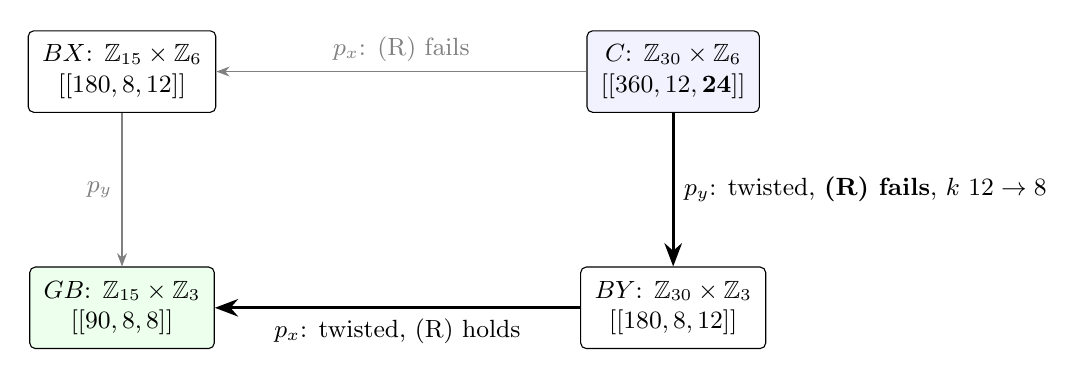
\begin{tikzpicture}[
  code/.style={draw, rounded corners=2pt, align=center, inner sep=5pt,
               font=\small},
  >={Stealth}]
\node[code, fill=blue!5] (C) at (7,3)
  {$C$: $\Z_{30}\times\Z_6$\\ $[[360,12,\mathbf{24}]]$};
\node[code] (BY) at (7,0) {$BY$: $\Z_{30}\times\Z_3$\\ $[[180,8,12]]$};
\node[code] (BX) at (0,3) {$BX$: $\Z_{15}\times\Z_6$\\ $[[180,8,12]]$};
\node[code, fill=green!7] (GB) at (0,0)
  {$GB$: $\Z_{15}\times\Z_3$\\ $[[90,8,8]]$};
\draw[->, very thick] (C) -- node[right, font=\small]
  {$p_y$: twisted, \textbf{(R) fails}, $k\ 12 \to 8$} (BY);
\draw[->, very thick] (BY) -- node[below, font=\small]
  {$p_x$: twisted, (R) holds} (GB);
\draw[->, gray] (C) -- node[above, font=\small\color{gray}]
  {$p_x$: (R) fails} (BX);
\draw[->, gray] (BX) -- node[left, font=\small\color{gray}]
  {$p_y$} (GB);
\end{tikzpicture}
\caption{The Bravyi-360 tower. The certification path (black) descends
$C \to BY \to GB$; the mirror path through $BX$ exists, commutes
(overflow square), and was never needed. All three order-2 decks of $C$
jump $k$ from $8$ to $12$: condition (R) fails on \emph{every} deck, in
every presentation --- the doubling theorem has nothing to say about this
code.}
\label{fig:bravyitower}
\end{figure}

\subsection{What descent found before the calculus existed}

The program's first campaign on this code (note A19) built the tower and
immediately hit the structural surprise: \textbf{(R) fails on every deck
of $C$} --- checked exhaustively across all presentations, using the fact
(program note A10) that such verdicts are code-level, not
presentation-level. After 157 consecutive historical covers had satisfied
(R), the first natural flagship outside the doubling template had
arrived. Everything the companion's safe sector needed was gone; what
remained was exactly the unconditional layer of
Sections~\ref{sec:transport}--\ref{sec:ledger}, and it already earned its
keep three times over:

\begin{itemize}[leftmargin=2em]
\item \emph{The ledger, measured.} $\operatorname{rank} p_{y*} = 6 =
  k/2$ despite the $k$-jump; $\dim (1+\sigma)_*\clH = 4 = k - \ov k$ for
  all three decks (the Bockstein equality's first flagship sighting);
  the doubly-new sector $\ker p_{x*} \cap \ker p_{y*}$ has dimension
  exactly $4$ and equals $\operatorname{im}(1+\sigma)_*$ deck-independently.
\item \emph{The upper bound is tower arithmetic.} Deep witness hunts
  found the cover's lightest known logicals at weight $24$ --- and they
  are \emph{transfer lifts}: $\tau_y(\text{weight-12 } BY
  \text{ logical})$, verified cycle-by-cycle, with the doubly-new sector
  bottoming at $32 = \tau_x \tau_y(\text{weight-8 } GB\text{ logical})$.
  So $d \leq 24$ constructively, and the tower's weight arithmetic
  ($24 = 2 \cdot 12$, $32 = 4 \cdot 8$) was visibly organizing the code.
\item \emph{Half the floor, cheaply.} Running the trisection at target
  $12$ --- census $BY$'s stabilizers to weight $11$ (seven translation
  classes: one hexagon, six at weight 10, \emph{no weight-8}), rung each,
  close the diagonal branch by $d(BY) = 12$ --- certified $d(C) \geq 12$
  in minutes: at the time, double the best bound for this code by any
  method.
\end{itemize}

Pushing the same architecture from target 12 to target 24 then met the
two walls that motivated Section~\ref{sec:secondshadow}. The dangerous
and seam censuses now needed weight $\leq 22$ \emph{at $n = 180$}: the
seam side priced at $3.3 \cdot 10^{13}$ enumeration nodes ($40$--$60$
hours), and the dangerous side's final band (weight-22 stabilizers of
$BY$, projected ${\sim}20{,}000$ classes) had stalled a SAT census at
151 classes. A month of engineering nibbled at the edges; the two-level
calculus deleted both walls in an afternoon.

\subsection{The two-level closure}

Descend the obligations one more rung, $BY \to GB$, and census at
$n = 90$ instead. The second-rung ledger is the R1 regime:
$\mathcal{K} = \ker p_{x*}$ (dimension 4, 15 nonzero classes in 3
translation orbits) sits \emph{inside} $\mathcal{S} = \Seam$ (dimension
6, 63 classes in 11 orbits), and $\mathcal{W} = p_{x*}(\mathcal{S})$ has
dimension 2 --- three nonzero classes, a single translation orbit ---
with $p_{x*}^{-1}(\mathcal{W}) = \mathcal{S}$: \emph{reachability is
decided one rung below}, so sectors (B) and (C) never need a class check.
The three sectors of Theorem~\ref{thm:secondshadow}, concretely:

\begin{itemize}[leftmargin=2em]
\item[\emph{(A)}] $[\beta] \in \mathcal{W}\setminus 0$: three $GB$-coset
  censuses to weight 22 --- minima 14; orbit populations $6$, $68$,
  $1{,}627$, $19{,}873$, $175{,}057$ at weights $14, 16, 18, 20, 22$ ---
  then lift fibers at caps $(22 - \wt\beta)/2 \leq 4$. Of $196{,}631$
  fibers only $13{,}404$ produced any lift at all ($\geq 93\%$
  carry-infeasible); every lift's rung passed.
\item[\emph{(B)}] $\beta = 0$: $b = \tau'(\gamma)$ with $\gamma$ a $GB$
  logical outside $\ker\tau'_*$ --- and $GB$'s logical census to weight
  10 (all 255 classes; $d(GB) = 8$ census-complete as a byproduct) shows
  38 relevant orbit classes, each rung-checked at its pinned overflow.
\item[\emph{(C)}] $\beta$ a nonzero $GB$ stabilizer: the $GB$ stabilizer
  census to weight 22 --- orbit populations $1$, $6$, $21$, $64$, $333$,
  $1{,}733$, $10{,}602$, $64{,}619$ at weights $6, 10, 12, \dots, 22$,
  with \emph{no weight-8 stabilizers} at all (the companion's weight-gap
  phenomenon, fourth sighting) --- fibers up, rungs on every lift. The
  predicted hard tail --- deep fibers over the lightest shadows, caps up
  to 8 --- had been priced at solver-hours; all 28 ran in $13.5$
  seconds.
\end{itemize}

And the stalled flat-22 dangerous residue --- weight-22 $BY$ stabilizers
with overflow 0 --- died twice over: its branch (B) is empty by the mod-4
test (Remark~\ref{rem:mod4}: $22 \equiv 2 \pmod 4$, zero compute), and
its branch (C) members are exactly the fibers already enumerated, each
finished by a flat-top rung ($27{,}152$ of them). The stalled census was
not completed --- it was \emph{generated}, as
Theorem~\ref{thm:secondshadow} promised, and the banked partial became a
membership cross-check.

\begin{center}
\small
\begin{tabular}{lll}
\toprule
obligation & before (per-level architecture) & after (two-level calculus)\\
\midrule
seam censuses, bands 18--22 & $3.3\cdot 10^{13}$ nodes, $40$--$60$ h &
$n{=}90$ censuses + fibers, ${\sim}10$ min\\
per-shadow floors & census-blocked & $49{,}855$ rungs, ms each\\
flat-22 residue & ${\sim}20$k-class census, stalled at 151 &
parity (0 s) + $27{,}152$ flat rungs\\
deep fibers & priced at solver-hours & $13.5$ s, all 28\\
$d(BY) = 12$ floor & $3.1$ h SAT ladders & $0.04$ s, same machine\\
$d(GB) = 8$ & $187$ s coset-SAT & $< 1$ s census\\
\bottomrule
\end{tabular}
\end{center}

\subsection{The verdict}

Total: $49{,}855$ rungs over ${\sim}274{,}000$ fibers, \emph{all pass},
${\sim}9.4$ minutes end-to-end, no SAT on the critical path; the
weight-24 transfer-lift witnesses close the top. By the assembly schema:
\[
d\bigl([[360,12,\leq 24]]\bigr) \;=\; 24, \qquad
\text{exactly --- the first determination of this code's distance.}
\]
It exceeds the strongest published solver-exact BB code by $25\%$ in
$n$ and $33\%$ in $d$, at a strictly more auditable grade. The
certificates are tight with slack one: the true minimum-weight logicals
sit at total overflow exactly one unit above the excluded strata.

\begin{sloganbox}
\textbf{The postscript that reframes doubling.} The certified values
satisfy $d(C) = 24 = 2 \cdot d(BY)$: the top level is a \emph{perfect
doubling} --- on a rung where (R) fails, $k$ jumps, and the doubling
theorem is not merely unproven but \emph{inapplicable}. Doubling, it
turns out, is a phenomenon that outruns the theorem that first captured
it; descent is how you certify it when the theorem's conditions desert
you. (The next tower stacks the opposite surprise: an (R)-rung that
\emph{fails} to double.)
\end{sloganbox}

% ==================================================================
\section{Worked instance II: IBM-288, or what (R) is actually for}
\label{sec:ibm288}
% ==================================================================

The second instance is the deliberate opposite of the first: a tower
where (R) holds on every rung, chosen to measure exactly what that buys
the calculus. The target is the strongest $k = 8$ code of IBM's 2026
discovery catalog,
\[
Y8: \quad \Z_{18} \times \Z_8, \qquad
A = 1 + xy^4 + x^{14}y, \qquad B = 1 + xy^2 + x^2y^7, \qquad
[[288, 8, 20]],
\]
with $d = 20$ known by MILP --- a solver value with no published
certificate. Its tower is same-axis, three storeys of $y$-halving:
\[
Y2\ (\Z_{18}{\times}\Z_2)\ [[72,8,6]]
\;\longrightarrow\;
Y4\ (\Z_{18}{\times}\Z_4)\ [[144,8,10]]
\;\longrightarrow\;
Y8\ [[288,8,20]],
\]
both upper rungs twisted, \textbf{(R) holding on both} with explicit
Bezout certificates ($1 + y^2 \in (A_4, B_4)$ and $1 + y^4 \in (A_8,
B_8)$), $k = 8$ born at the bottom storey and carried up unchanged. The
distance arithmetic already tells a story the walls section will pick
up: the first rung loses distance ($10 = 2\cdot 6 - 2$, exactly the
\emph{deficit wall} value), the second doubles perfectly ($20 = 2 \cdot
10$) --- one tower, both extremes, so whatever sets the ratio acts per
rung.

\subsection{Where the doubling template actually stalled}

Because (R) holds, this tower was first attacked with the companion's
template aimed at the top rung (program note A20), and five of its six
obligations fell quickly: the base floor $d(Y4) = 10$; the dangerous
census (1,655 stabilizer classes to weight 18, later re-derived four
independent ways) with all fiber-pinned floors; the Bezout certificate;
the weight-20 transfer-lift witness. The sixth --- the safe floor ---
produced the campaign's structural discovery: \textbf{the naive seam
floor is false.} The 15 seam classes collapse into two translation
orbits (sizes 12 and 3), and the 12-orbit's coset contains a
\emph{weight-18 element} --- sitting exactly at the wall value $2 d(Y4)
- 2 = 18$. Not a counterexample to $d = 20$ (the floor is sufficient,
not necessary), but fatal to the template's safe half as stated. The
repair is the \emph{lift-aware} floor of
Theorem~\ref{thm:trisection}(ii): census every light coset element, and
rung each element's fiber. The SAT lane then spent ${\approx}12.7$ hours
certifying 278 elements of \emph{one} orbit --- census not exhausted ---
and $3.8$ inconclusive hours on the other. Roughly $16.5$ solver-hours,
for a partial answer. That was the open state for three weeks.

\subsection{The calculus port, and the (R)-collapse}

The two-level machine closed it in a session. Direct lane: one
three-offset coset-BZ pass at $n = 144$ ($6.6\cdot 10^{10}$ nodes,
$61$ s) censused the stabilizers \emph{and} both seam cosets
simultaneously: the 12-orbit coset holds exactly $1{,}680$ elements of
weight $\leq 18$ ($\{14{:}\,6,\ 16{:}\,84,\ 18{:}\,1{,}590\}$ --- the
dying SAT census had been two translation classes short), and the
3-orbit coset is \textbf{empty} below 20 --- the naive floor was
\emph{true} there all along, which retroactively explains the
inconclusive probe. The $1{,}680$ per-element rungs all passed in
$1.8$ seconds ($94.6\%$ at cap 1). Every remaining solver input was
re-derived by census or tower in seconds ($d(Y2) = 6$, the $Y4$ logical
floor, the dangerous floors --- $1{,}655$ deterministic rungs agreeing
with $1{,}655$ banked SAT verdicts), leaving
\[
d\bigl([[288,8,20]]\bigr) = 20, \qquad
\text{${\sim}105$ s of critical-path compute, no SAT} ,
\]
an ${\approx}600\times$ improvement over the partial solver campaign,
and the program's first certified $d = 20$ on a \emph{previously
published} code. (Its first certified $d = 20$ outright had landed four
days earlier on two $[[360,4,20]]$ codes the program itself constructed
by doubling --- a priority footnote the notes keep straight with some
care, and so do we.)

The descent lane then re-derived the same $1{,}680$-element census from
$n = 72$ data --- and here is what (R) is \emph{actually for}. This
tower sits in regime R2: $\mathcal{S} \cap \mathcal{K} = 0$, and
$p'_*$ is injective on $\Seam$, so each of the 15 seam classes pins to
a \emph{single} bottom-code coset --- the trisection collapses to
sector (A) alone, one branch, one target coset per class. The
$105{,}328$-element bottom coset census fibered up ($90.6\%$
carry-infeasible) to exactly the $1{,}680$ direct elements; the 3-orbit
side produced $8{,}460$ lifts, none in the seam --- emptiness re-derived
from below.

\begin{keyidea}[What (R) buys, measured]
Contrasting the two instances isolates (R)'s true role in descent.
Soundness never consumed it: the Bravyi tower closed with (R) failing
everywhere. What (R) delivers is \emph{collapse} --- $k$ preserved, the
deck invisible on classes, base-side exactness ($\ker\tau_* =
\Seam = \imD$), and through those, regimes R2/R3 where the second-level
trisection loses one or two branches. In the doubling theorem (R) was a
load-bearing wall; in the descent calculus it is a discount coupon.
\end{keyidea}

Two further port lessons, recorded because later instances leaned on
them: the same-axis tower degenerates the overflow square (only one
descent order exists) and offers a composite $\Z_4$ deck --- and neither
mattered, since \emph{iterated $\Z_2$ sufficed for everything}; and the
$2^{k}$-sector rung dispatch costs nothing at $k = 8$ (256 sectors),
foreshadowing that $k$-genericity, not (R), governs the dispatch
(confirmed at $4{,}096$ sectors in the next section).

% ==================================================================
\section{Worked instance III: the record code in 31 seconds}
\label{sec:bb288}
% ==================================================================

The capstone is the running tower itself: the published record
$[[288,12,18]]$, descending through gross and bb72 to the fully
enumerable $[[36,8,4]]$. It is the strongest solver-exact BB code in
the literature, and it had been \emph{solver-hostile} in-program: direct
UNSAT floor queries at $n = 288$ were intractable in every lane the
program tried, and two dedicated SAT-acceleration campaigns closed
negative-with-data. The conditions-map survey of
Section~\ref{sec:conditions} rated its four-level tower green on every
gate and ranked it the \#1 port; the closure (note A36) landed the same
day, and every projected cost came in on the money.

\subsection{The closure, compressed}

The rung ledger: top rung twisted-(R) (the $y^7$ twist), middle rung
untwisted-(R) --- \emph{the companion's own gross-over-bb72 rung, now a
middle storey} --- bottom rung twisted-non-(R) ($k$ drops $12 \to 8$).
The lower pair sits in regime R3: $\Seam = \ker p_{x*}$ \emph{exactly},
so $\mathcal{W} = 0$ and sector (A) is empty one rung down --- no
bottom-coset censuses exist at all, the structural opposite of the
IBM-288 collapse. The seam space at the gross level has dimension 6:
63 classes in five translation orbits, so five coset offsets cover the
entire safe sector.

The direct closure is one six-offset BZ pass at $n = 144$ ($7.5 \cdot
10^9$ nodes, ${\sim}25$ s: stabilizer census and all five seam-orbit
cosets in a single walk) plus the rung layer ($3.2$ s):

\begin{itemize}[leftmargin=2em]
\item \emph{Dangerous:} 469 stabilizer orbit classes to weight 16
  ($\{6{:}1,\ 10{:}6,\ 12{:}33,\ 14{:}54,\ 16{:}375\}$; no weight-8
  stabilizers --- the gap's fifth sighting), all 469 rungs pass at caps
  $\leq 5$, with the full $2^{12} = 4{,}096$-sector dispatch validated
  sector-by-sector and costing nothing.
\item \emph{Seam:} 395 coset elements to weight 16 ($\{12{:}3,\
  14{:}18,\ 16{:}374\}$) --- minima at $12 = d(\mathrm{gross})$, so the
  naive floor fails here too --- all 395 per-element rungs pass ($94.7\%$
  flat-top). A convention tripwire armed the whole census: any seam
  element below 12 would have contradicted a kernel-checked theorem
  (next item), so the census doubles as a consistency test against Lean.
  It stayed silent.
\item \emph{Diagonal:} $\wt v \geq 2\, d(\mathrm{gross}) = 24$, and
  here the tower consumed its most distinguished input: $d(\mathrm{gross})
  = 12$ \emph{at kernel-checked tier} --- the companion's theorem, as
  machine-verified in Lean --- imported with zero new obligations (the
  branch needs only $d \geq 10$). Per-level inputs compose at any tier
  at or above certificate grade, and the assembly inherits the weakest
  tier: certificate overall, with one leg stronger.
\end{itemize}

The witness search was run as an exhaustive ladder over strata,
\emph{armed in both directions}: any find below 18 would refute the
published record; silence at every stratum would refute $d = 18$ itself.
One of the two had to fire. The negatives came first and are structure,
not failure: no weight-18 logical exists at overflow 1 over \emph{any}
weight-16 shadow, nor at overflow 2 over any weight-14 shadow. The first
hit landed at the lightest seam band: a weight-18 logical over a
weight-12 seam element at overflow 3 --- and that seam element is itself
the $\tau$-lift of a \emph{weight-6 bb72 logical}. The record code's
minimum-weight logical sits over the diagonal of the diagonal:
$d$-attainment projecting onto $d$-attainment two levels down (measured
here, not claimed universal --- the previous tower's witness had a
different profile, and the notes flag exactly that).

\[
d\bigl([[288,12,18]]\bigr) = 18:
\quad \text{${\sim}31.4$ s + $0.4$ s witness, no SAT anywhere.}
\]

An independence lane ($1.0$ s) re-derived both gross-level censuses from
$n = 72$ data through the R3 identity --- key-set equality, 469 and 114
orbit classes respectively --- and threw off one more gift: the full
bb72 cycle census to weight 8, making $d(\mathrm{bb72}) = 6$
\emph{census-complete}, solver-free. That value is an input to the
companion's own story (its Input T-A is the statement that nothing
lighter exists); the tower repaid its ancestor.

\subsection{Three closures, one trend}

\begin{center}
\footnotesize
\begin{tabular}{lllll}
\toprule
instance & tower & regime & critical path & prior state\\
\midrule
$[[360,12,\leq24]] \Rightarrow d{=}24$ & 3 levels, mixed, top $\neg$(R)
& R1 & ${\sim}9.4$ min & open ($40$--$60$ h priced)\\
$[[288,8,20]] \Rightarrow d{=}20$ & 3 levels, same-axis, all-(R) & R2 &
${\sim}105$ s & ${\approx}16.5$ h SAT, partial\\
$[[288,12,18]] \Rightarrow d{=}18$ & 4 levels, mixed, one $\neg$(R) & R3
& ${\sim}31$ s & solver-hostile, no floor\\
\bottomrule
\end{tabular}
\end{center}

The trend is the right way around: \emph{deeper towers make the calculus
cheaper}, because the censuses --- the only super-polynomial ingredient
--- run at the bottom, and each extra storey halves the bottom. The
record code, at the same $n$ as IBM-288 but with a four-level tower, cost
a third as much; and its $n = 36$ bottom, pinned in advance by full
enumeration, was never even needed for the floor ($n = 144$ censuses
were already trivial) --- deeper levels served \emph{independence}, not
necessity. Meanwhile the three closures exercised three of the four
regimes, on twisted and untwisted rungs, mixed and same axes, (R) and
non-(R) --- the portability claims of the calculus are not projections;
each was measured on the next structurally different tower.

% ==================================================================
\section{The conditions map: what the calculus needs, and what it costs}
\label{sec:conditions}
% ==================================================================

After three closures the program did the disciplined thing: it stopped
closing instances and mapped the method --- decomposed the calculus into
layers, pinned each layer's exact hypothesis at its honest grade
(theorem / measured / instance data / cost gate), and then \emph{measured
every gate} on an eleven-tower, twenty-two-rung docket that had to
reproduce the closed instances' numbers before screening anything new
(note A35). This section is that map, compressed.

\subsection{Hard requirements: exactly two}

\begin{description}[leftmargin=2em,style=nextline]
\item[C1: a free $\Z_2$ deck --- that is, $2 \mid \lvert G \rvert$.]
  The slice identity and the sheet decomposition are two-sheet
  arithmetic; an odd-order deck offers no $\F_2$ transfer (the
  telescoping $1 + \sigma + \cdots + \sigma^{p-1}$ has no
  characteristic-2 magic). Odd factors of $\lvert G\rvert$ are inert ---
  they only set the size of the bottom code. Odd-$\lvert G \rvert$ codes
  are simply outside: for them the program's older per-level machinery
  (fibering engines, coset certificates) remains the only lane.
\item[C2: the two-block group-algebra CSS shape, with a central deck.]
  Every proof in Sections~\ref{sec:transport}--\ref{sec:trisection} used
  exactly two properties of $\sigma$: order two and centrality. Beyond
  abelian groups (Section~\ref{sec:finding}) the deck must be a
  \emph{central} involution; and the $X$--$Z$ transpose duality (which
  let us work one-sided) is BB-specific --- without it, run both sides.
\end{description}

Everything else in the doubling theorem's condition list is demoted:
parity of $\wt A, \wt B$ is a \emph{simplifier} (halved strata, the
mod-4 scalpel, even distances --- lost gracefully if a weight is even);
(R), $\sigma_* = \mathrm{id}$, base-side exactness, regime identities,
weight gaps, light-logical concentration are \emph{discounts} measured
per instance; none is a precondition. The one-sentence summary the
program's handoff uses: \emph{soundness needs nothing else}.

\subsection{Feasibility: five numbers}

Whether a \emph{particular} tower closes at a \emph{particular} target is
governed by five measurable gates; the screen prices them per tower
without running the closures.

\begin{description}[leftmargin=2em,style=nextline]
\item[G1 --- bottom-census nodes.] The BZ node count
  $\sum_{s\leq r_1}\binom{\kappa}{s} + \sum_{s\leq r_2}\binom{\kappa}{s}$
  at the bottom level, $\kappa = n/2 - k/2$, $r_1 + r_2 + 1 = W$. The
  formula is exact (validated $\times 1.00$ against production anchors);
  the demonstrated envelope is ${\sim}2\cdot 10^{11}$ nodes $\approx$
  minutes. Deep towers help \emph{here}: each storey halves $\kappa$
  inside binomials. (The quieter frontier is census \emph{storage}:
  orbit populations grow $9$--$24\times$ per weight band near the bulk.)
\item[G2 --- fiber caps.] $\mathrm{cap} = (W - \mu)/2$ at the lightest
  nonzero shadow weight $\mu$ ($\leq \wt A + \wt B = 6$ on the whole
  docket). Demonstrated: cap 8. The cap grows linearly in the target ---
  this, not the census, is what walls off the deepest questions.
\item[G3 --- sector dispatch.] $2^{k(\base)}$ classes per dangerous
  rung; measured free through $k = 12$ ($4{,}096$ sectors).
\item[G4 --- the emptiness rate is a bonus, never a budget line.] See
  Section~\ref{sec:fibers}: real ($86$--$97\%$ in production), and
  provably not predictable before the census exists.
\item[G5 --- the diagonal ceiling.] The branch-(0) floor is
  $2\,d(\text{next level down})$, so certifying $d_t$ needs $d_t \leq
  2\,d(M)$ at \emph{every} storey, with the bottom $d$ pinned by census
  or outright enumeration. Every closed instance satisfies it with room;
  it is the first thing to check on a new tower.
\end{description}

\subsection{The screen's verdicts, including the honest ones}

The 22-rung screen confirmed every structural law of
Section~\ref{sec:ledger} ($22/22$), realized all four regimes, and
returned cost verdicts --- \emph{cost} verdicts, the note is careful to
say, not proofs:

\begin{itemize}[leftmargin=2em]
\item \emph{Green and executed:} the record code's four-level tower
  (Section~\ref{sec:bb288}; every projection landed on the money).
  \emph{Green and waiting:} a $[[336,12,12]]$ full closure over a third
  group shape (cheapest on the docket, ${\lesssim}10^9$ nodes); the
  gross-over-bb72-over-$[[36,8,4]]$ retrospective (regime R4, both
  distances known --- the reader's exercise); and the \emph{freeze
  question} for a $[[720,4,{\geq}20]]$ re-doubled tower at $W = 18$--$22$
  --- which would decide, at certificate grade, whether the same-axis
  re-double freeze the program has always observed
  (Section~\ref{sec:walls}) holds for the first $d = 20$ tower.
\item \emph{Red, and quantified:} that same $[[720]]$ tower's full
  doubling question ($d = 40$?) needs fiber caps of 16 --- twice
  anything demonstrated. And the one flagship the calculus honestly does
  not reach: Bravyi et al.'s $[[756,16,\leq 34]]$. Its group's
  $2$-part is a single $\Z_2$ ($v_2 = 1$): the tower has one storey, the
  bottom census sits at $10^{22.6}$ nodes, and no deeper tower exists to
  push it down. The one-deck reduction helps by five orders of magnitude
  and misses by eleven. The honest statement, quoted from the note:
  the gap ``needs new reductions, not more compute.''
\end{itemize}

% ==================================================================
\section{Finding towers, and what else descends}
\label{sec:finding}
% ==================================================================

The calculus assumes a tower. This section is about where towers come
from, what descends besides distance, and how far past bivariate abelian
codes the frame reaches.

\subsection{Deck inventory and detection}

For a BB code the deck inventory is trivial to list --- at most three
order-2 monomials, and the full tower is the $2$-part of $G$, one
$\Z_2$ at a time in any order. What takes actual work is recognizing a
\emph{presentation}: given the top code as a raw polynomial pair, finding
the change of coordinates (group re-decomposition, automorphism ---
including the mixing ones --- block swap, translations) under which a
chosen deck's quotient becomes visible in windowed form. The program
packaged this as a single driver (\texttt{descend(code)}): input a BB
code, it enumerates the decks, hunts presentations over the full
automorphism sweep, runs the $k$-gate (Theorem~\ref{thm:A12}: one rank
computation decides (R) per deck), and reports per-deck verdicts with
certificates. Two of its validation runs are already familiar in
spirit: on the IBM-288 code it auto-reconstructs the $Y4$ base and
\emph{independently rediscovers}, in two seconds, the weight-18
seam-coset element that broke the naive safe floor; on the record code
it reproduces the same-axis freeze refutation. Run across IBM's
98-class discovery catalog it sorted the whole table in
${\sim}24$ minutes --- most valuably its negatives: $30$ catalog codes,
including both distance-record flagships, are provably outside the
literal-lift \emph{doubling} route (k-jumps, twisted-only decks, or
certificate rejections). Codes outside the doubling route are not
outside the \emph{descent} route; that asymmetry is the point of this
document.

\subsection{\texorpdfstring{$k$}{k} descends first}

Distance is the hard passenger; the logical count $k$ rides the tower
under complete control, and the control theorems are the program's
(all Lean-backed, Section~\ref{sec:trust}):

\begin{itemize}[leftmargin=2em]
\item \emph{One rung}: the $k$-ladder $\ov k \leq k \leq 2\ov k$
  (Corollary~\ref{cor:kladder}), the Bockstein equality
  (Theorem~\ref{thm:bockstein}), and the (R) trichotomy
  (Theorem~\ref{thm:A12}).
\item \emph{Whole towers}: for a $\Z_{2^r}$ tower, deck-triviality at
  the \emph{top} already forces $k$ constant at \emph{every} level ---
  equivalently $1 + \sigma \in (A,B)$, one ideal-membership certificate
  covering the entire ladder (program note A13; the proof's engine is a
  clean divisibility lemma, ``$\varepsilon$-torsion is
  $\varepsilon$-divisible,'' in the local ring $\F_2[\varepsilon]$).
  On the gross $x$-ladder one certificate --- the companion's
  $(1+x^2)B^2 = 1+x^6$, which never mentions the $x$-order --- pins
  $k = 12$ at every level up through $[[576,12,\cdot\,]]$.
\item \emph{The birth pattern.} Sweeping every deck of every code in the
  published tables: each $k = 12$ flagship acquires its $k$ at exactly
  one deck-nontrivial rung and carries it through (R)-rungs thereafter.
  Gross and the record code both root at bb72; bb72's own $k = 12$ is
  born one storey further down; Bravyi-360's is born at its top rung.
  The towers are not an analytical trick imposed on the codes --- the
  codes' parameters are visibly \emph{organized} by their towers.
\end{itemize}

\subsection{The construction direction is genuinely harder}

Descent's robustness invites a converse hope: given a good base, must a
distance-doubling cover exist? \textbf{No.} The program's A10 screen
formalized the search space (four extension classes per base --- two
axes, a diagonal, a split class --- times all sheet-assignment
\emph{twists} of the polynomials) and found thirteen certified
counterexample bases whose \emph{entire} 256-cover descent space fails:
every cover either drops $k$ or exhibits an explicit light logical. The
same screen showed twists genuinely matter for construction --- two
gross siblings that fail every literal-lift cover are rescued by twisted
covers, one of them by no literal lift of \emph{any} equivalent
presentation. Constructing covers is a search through a
presentation-sensitive space with real dead ends; \emph{descending} a
given cover is deterministic. The asymmetry is why this document's
direction of travel --- down --- is the dependable one.

\subsection{Beyond bivariate: the non-abelian audit}

How much of the frame survives when $G$ stops being abelian? The
transport layer never used commutativity of $G$ --- only centrality and
order 2 of $\sigma$ (the footnote of Section~\ref{sec:decks}). The
program tested this on the published \emph{mitten codes}
(non-abelian lifted-product codes, arXiv:2607.28795): of the eight
published instances, exactly the three whose group centers have even
order carry central involutions, hence decks; all three descend. The
regime is the $k$-ladder's \emph{other} extreme: mitten towers are
$k$-\emph{doubling} ($k = 2\ov k$ on every rung, forced by the
construction's $k = \lvert G\rvert$), the deck acts maximally on
classes, and descent \emph{loses} distance ($d < 2\ov d$ on three of
four measured rungs) --- the structural complement of the $k$-preserving
BB towers, measured at exactly the upper bound the (BB-proved) ladder of
Corollary~\ref{cor:kladder} names. (The ladder's proof used the BB
transpose duality; its non-abelian re-derivation is on the program's
queue, with the measured values already voting yes.) Two of the
four rungs echo the deficit wall at $2\ov d - 2$
(Section~\ref{sec:walls}).

The audit also demonstrated descent's value as \emph{due diligence}: the
descent computation on the published $[[300,60,14]]$ table row found the
row's polynomial data describes a different code entirely --- distance
6, one generator matrix rank-deficient against the paper's own
definition --- while the paper's shipped artifact is the real
$[[300,60,14]]$; a reportable erratum surfaced by trying to descend a
table. (A cross-check of that family: the $[[150,30,10]]$ sibling's
distance was later certified end-to-end \emph{in Lean} by this program
--- the first formally verified non-abelian qLDPC distance --- so the
family's numbers now rest on more than solver output twice over.)

% ==================================================================
\section{Walls, deficits, and the failure gallery}
\label{sec:walls}
% ==================================================================

A calculus that computes exact distances down towers accumulates, as a
byproduct, the best available data on the question the doubling theorem
begged: \emph{when} does a rung double, and by how much does it miss?
This section collects the phenomenology, the one theorem, and the
program's negative results --- stated with the same care as the positive
ones, because several are protections against errors the program
actually committed.

\subsection{The deficit ledger and the wall theorem}

Define a rung's \emph{deficit} as $2\,d(\base) - d(\cov)$. The certified
values now span:

\begin{center}
\small
\begin{tabular}{llll}
\toprule
rung & $d(\base) \to d(\cov)$ & deficit & note\\
\midrule
bb72 $\to$ gross & $6 \to 12$ & $0$ & the companion's theorem\\
$Y4 \to Y8$ (IBM-288) & $10 \to 20$ & $0$ & perfect, above a wall rung\\
$BY \to$ Bravyi-360 & $12 \to 24$ & $0$ & perfect, (R) failing\\
$[[36,8,4]] \to$ bb72 & $4 \to 6$ & $2$ & \emph{the wall}\\
$Y2 \to Y4$ (IBM-288) & $6 \to 10$ & $2$ & \emph{the wall}\\
$GB \to BY$, $GB \to BX$ & $8 \to 12$ & $4$ & both axes equal\\
gross $\to$ record bb288 & $12 \to 18$ & $6$ & (R) holds; floors fail\\
mitten $[[150]]{\to}[[300]]$, $[[270]]{\to}[[540]]$ & $8 \to 14$,
$10 \to 18$ & $2$ & non-abelian echoes\\
\bottomrule
\end{tabular}
\end{center}

Every deficit is even --- that much is cycle parity --- and the value
$2$ recurs suspiciously. The one theorem in this territory (program note
A17, Lean-packaged) explains the recurrence. For odd-weight pairs on
(R)-rungs, define the base's \emph{safe-sector distance} $d_{\mathrm{safe}}$
as the minimum weight over cycles whose class lies in $\imD \setminus 0$
--- by Proposition~\ref{prop:seamvsimD}, the minimum weight of a base
logical \emph{that dies in the cover}. Then $d_{\mathrm{safe}}$ is even;
the doubling template's safe half is viable iff $d_{\mathrm{safe}} \geq
2d$; and if it is \emph{not} viable, then $d_{\mathrm{safe}} \leq 2d - 2$
--- \textbf{the wall value $2d - 2$ is the unique maximal failing
value}, nothing between $2d - 1$ and viability being achievable, by
parity alone. Moreover the failure transports: a cover that fails to
double through its safe sector hands the base a light safe-class witness
at no weight cost ($d_{\mathrm{safe}} \leq \tilde d_{\mathrm{safe}}$,
the pushforward mechanism). The wall is genuinely attained (the two
wall rows above); naive safe floors inside otherwise-healthy towers fail
through light seam elements, and the first such element ever surfaced sat
at exactly the wall value ($18 = 2\,d(Y4) - 2$, on the IBM-288 tower ---
the complete census later found elements down to weight 14 on that
orbit, and the sibling orbit \emph{empty}: the failure is per-orbit, not
per-code); and the echo in the non-abelian, $k$-doubling mitten family
--- both regime knobs flipped --- upgrades it, in the note's words, from
bivariate curiosity toward a generic 2-cover phenomenon. What sets the deficit
when it is \emph{not} the wall ($4$? $6$?) is open, and the deck survey's
freeze observation --- every proven double, re-doubled on the same axis,
keeps its old distance --- is the standing conjecture the $[[720]]$
freeze certification (Section~\ref{sec:conditions}) would test at
certificate grade.

\subsection{A cautionary tale the program paid for}

The wall was first ``observed'' as: \emph{safe floors stall at exactly
$2d - 2$}. That sharp premise turned out to be a measurement artifact,
and the note that proves the wall theorem also retracts the observation
that motivated it: the old sweeps had recorded \emph{the weight of the
first extracted SAT model} at a query bound --- an upper bound on the
minimum, not the minimum. Corrected ladders moved several ``exactly
$2d-2$'' readings strictly below the wall. Out of the episode came two
standing rules quoted verbatim across later notes, both already visible
in this document's design:

\begin{itemize}[leftmargin=2em]
\item \emph{Never report solver witness weights as floors.} Witnesses
  certify ``$\leq$''; only complete enumeration or UNSAT-with-certificate
  certifies ``$\geq$'' --- and at cover scale the latter is priced out,
  which is why descent relocates every ``$\geq$'' obligation down the
  tower.
\item \emph{Hits are decisive; timeouts are not evidence.} A dead
  witness-side query at $n = 360$ says nothing. The program retired
  blind top-level SAT entirely: the top code is for finding witnesses,
  the tower is for excluding everything else.
\end{itemize}

\subsection{Falsified folk-claims}

Each of the following sounded plausible, circulated briefly inside the
program, and is now refuted with a certificate; recorded so no reader
rebuilds on them.

\begin{itemize}[leftmargin=2em]
\item \emph{``Light logicals concentrate outside $\operatorname{im}
  p_*$.''} True at six measured sites in a row, then false at the
  seventh (the bb72-over-$[[36,8,4]]$ rung: 9 of 27 minimum-weight
  classes sit \emph{inside}). Where it holds it is instance luck;
  nothing in this document consumes it.
\item \emph{``The fiber emptiness rate can be estimated by cheap
  sampling.''} No: shallow-sampled rates read $0$--$17\%$ where the
  census populations read $86$--$97\%$. Emptiness lives deep in the
  census tail.
\item \emph{``The tower wins by compressing censuses.''} Measured
  compression of existing censuses under second-shadow quotienting is a
  modest $2.2$--$2.7\times$. The win is that census \emph{generation}
  moves to the bottom ($\kappa$ halves inside binomials) and most fibers
  are empty --- do not sell the calculus as a compression statement.
\item \emph{``There are no weight-8 stabilizers'' (the companion's
  weight-gap, as a law).} Holds at gross, $Y4$, $BY$, $GB$, and bb72;
  fails at $Y2$ and $[[36,8,4]]$. Cite per instance only.
\item \emph{``Witness profiles transfer between towers.''} IBM-288's
  minimum sits in the diagonal sector; the record code's sits over a
  seam element two storeys deep. The witness ladder must be run, armed
  in both directions, every time.
\end{itemize}

% ==================================================================
\section{Trust, and the formal frontier}
\label{sec:trust}
% ==================================================================

The program grades every claim on an explicit ladder, and this document
has used its top three grades; here is the whole ladder at once,
bottom-up, so the headline results sit in honest relief:

\begin{center}
\small
\begin{tabular}{lll}
\toprule
grade & certifies & example in this document\\
\midrule
ISD estimate & ``$\leq$, believed tight'' & mitten quotient distances\\
witness grade & ``$\leq$'', verified operator & every upper bound here\\
solver grade & UNSAT rounds, no artifact & the retired prior state\\
\textbf{certificate tier} & counting-invariant enumerations &
\textbf{all three headline floors}\\
kernel-checked & Lean, axiom-audited & $d(\mathrm{gross}) = 12$;
the ledger theorems\\
\bottomrule
\end{tabular}
\end{center}

Two design points. First, the ladder measures \emph{trust base}, which
the program keeps strictly orthogonal to the analytic-vs-computational
axis: the gross theorem is \emph{analytic} (surveyable case tables,
zero load-bearing computation) \emph{and} kernel-checked; the descent
results are \emph{computational by design} --- certified enumeration
\emph{is} the method --- and certificate-tier. Neither subsumes the
other, and the program's Goal-1 constraint (``fully analytic only'') was
never relaxed for descent; descent opened a second front with a
different currency. Second, the tiers \emph{compose}: the record-code
assembly consumed the kernel-checked gross theorem as its diagonal
branch and inherits the weakest tier of its legs --- certificate overall,
one leg stronger.

\paragraph{The Lean frontier.}
What is kernel-checked today, in the QECLean library: the entire
transport and ledger layer (Sections~\ref{sec:transport}
and~\ref{sec:ledger}) in parametric form (deck towers, the Bockstein
equality with twisted decks, the deficit-wall theorem, the Bezout
certificate lemma --- all axiom-clean); the companion's theorems (gross
unconditional; the pair72 and cover300 instances); and, for the record code, the same-day two-tier
packaging of the Section~\ref{sec:bb288} closure: the first
\emph{twisted} cover-data instance in the library (the $y^7$ twist costs
nothing --- the bundled obligations are pushforward identities, all
kernel \texttt{decide}s), the weight-18 witness half unconditional, the
diagonal branch discharged from the library's gross theorem with zero
new obligations, and the two certificate layers (dangerous and seam
floors) as named hypotheses --- the exact interface where a
census-carrying certificate species would slot in. That species is the
open engineering: BZ counting certificates and rung dispatches have
shipped Lean analogues from earlier campaigns, and the program's mitten
$[[150,30,10]]$ certification --- distance and all, the first formally
verified non-abelian qLDPC code --- demonstrates that census-scale
sweeps fit inside kernel-checked builds. Nothing on the path is open
mathematics; it is budgeted work.

\paragraph{Reproduction.}
Every closure in this document ships as scripts plus data plus a
verification map --- a claim-by-claim table pairing each assertion with
the check that re-derives it --- and every session note carries a
falsified-claims ledger recording what that session briefly believed and
then killed. A reader who wants to \emph{re-run} rather than re-read
starts at the verification maps of notes A32, A33, and A36.

% ==================================================================
\section{Where to read more}
\label{sec:further}
% ==================================================================

All sources live in the \texttt{qec-lab} research repository (paths
relative to \texttt{experiments/bb\_lab/}) and the \texttt{QECLean}
library.

\begin{center}
\footnotesize
\begin{tabular}{@{}>{\raggedright\arraybackslash}p{0.47\textwidth}@{\quad}>{\raggedright\arraybackslash}p{0.47\textwidth}@{}}
\toprule
what & where\\
\midrule
the tower slice calculus (transport, trisection, engine, Bravyi
closure) & \texttt{notes/A32\_tower\_slice\_calculus.md}\\
the IBM-288 port; what (R) buys, measured &
\texttt{notes/A33\_ibm288\_d20\_certificate.md}\\
the record-code closure in 31 s &
\texttt{notes/A36\_bb288\_d18\_certificate.md}$^\ast$\\
the conditions map; the 22-rung screen &
\texttt{notes/A35\_tower\_calculus\_generality.md}$^\ast$\\
the towers before the calculus (M12; the seam discovery) &
\texttt{notes/A19\_*.md}, \texttt{notes/A20\_*.md}\\
BZ censuses; the census-side trisection &
\texttt{notes/A28\_light\_classification\_theory.md}\\
coset-BZ, rungs, the \texttt{doubling\_certify} front-end &
\texttt{notes/A30\_coset\_bz\_doubling\_certificates.md}\\
(R) $\Leftrightarrow$ $k$ $\Leftrightarrow$ Bezout; deck towers;
Bockstein & \texttt{notes/A12\_*.md}, \texttt{notes/A13\_*.md}\\
the deficit wall & \texttt{notes/A17\_deficit\_wall.md}\\
descent covers and twists (the existence direction) &
\texttt{notes/A10\_descent\_twist\_screen.md}\\
the non-abelian audit & \texttt{notes/A26\_mitten\_descent.md}\\
Lean: transport layer and instances &
\texttt{QEC/Stabilizer/Framework/} \texttt{Homological/}
(\texttt{BBCover}, \texttt{BBDoubling}, \texttt{BBDeckTower},
\texttt{BocksteinLift}, \texttt{BBBocksteinTransport},
\texttt{BBDeficitWall}, \texttt{BBTargetFloor})\\
Lean: the record-code package &
\texttt{QEC/Stabilizer/Codes/} \texttt{BivariateBicycle/Bb288/}\\
\bottomrule
\end{tabular}
\end{center}

\noindent{\footnotesize $^\ast$On the research branch
\texttt{claude/tower-slice-calculus-generalize-410ed1} at the time of
writing.\par}

\medskip

The reader who wants to \emph{do} something is pointed one more time at
the exercise the notes themselves queued: run the calculus on the
running tower's lower pair --- certify $d(\mathrm{gross}) = 12$ or
$d(\mathrm{bb72}) = 6$ through the $[[36,8,4]]$ bottom. It is regime R4,
the one no headline instance exercised; both answers are known (one of
them kernel-checked), every census fits in seconds, and it would
complete the regime table. All the machinery you need is in
Sections~\ref{sec:transport}--\ref{sec:engine}.

\begin{thebibliography}{9}
\bibitem{bcgmry} S.~Bravyi, A.~W. Cross, J.~M. Gambetta, D.~Maslov,
P.~Rall, T.~J. Yoder, \emph{High-threshold and low-overhead
fault-tolerant quantum memory}, Nature \textbf{627}, 778--782 (2024);
arXiv:2308.07915. Tables cited: the BB code table, including
$[[288,12,18]]$ and $[[360,12,\leq 24]]$.
\bibitem{ibmdiscovery} The IBM bivariate-bicycle discovery catalog,
arXiv:2606.02418 (2026). Cited for its Table II ($[[288,8,20]]$,
MILP-exact) and its code tables swept in Section~\ref{sec:finding}.
\bibitem{mitten} \emph{High-rate qLDPC processors}, arXiv:2607.28795
(2026). The non-abelian lifted-product (``mitten'') codes of
Section~\ref{sec:finding}.
\end{thebibliography}

\appendix

% ==================================================================
\section{Notation summary}
% ==================================================================

\begin{center}
\small
\begin{tabular}{lll}
\toprule
symbol & meaning & where\\
\midrule
$C(v) = Av_L + Bv_R$ & syndrome map; cycles $= \ker C$ &
\S\ref{sec:recap}\\
$S(z) = (Bz, Az)$ & stabilizer map; stabilizers $= \operatorname{im} S$ &
\S\ref{sec:recap}\\
$\clH$, $[v]$, $k$ & class space, class, its dimension &
\S\ref{sec:recap}\\
$K = \ker S$ & relations (metachecks); $\dim K = k/2$ &
\S\ref{sec:recap}\\
$\sigma$, $p$, $\tau$, $e_0$, $e_1$ & deck, fold, transfer, sheet
embeddings & Def.~\ref{def:deck}\\
$\ov{(\cdot)}$ & base-level object ($\ov A = p(A)$, $\ov C$, $\ov k$,
\dots) & \S\ref{sec:decks}\\
twisted lift & cover polynomial terms carrying $\sigma$ &
Def.~\ref{def:twist}\\
$(1+\sigma)f = \tau(p(f))$ & the master identity & \eqref{eq:master}\\
$b = p(v)$; overflow $m$ & shadow; $\wt v = \wt b + 2m$ (slice identity)
& Lem.~\ref{lem:slice}\\
$\kappa(b)$; $\ov C(v_0) = \kappa(b)$ & lift carry; the carry equation &
Thm.~\ref{thm:carry}\\
$\mathrm{Fib}(b)$ & lift fiber: solutions, a coset of $\ker \ov C$ &
Thm.~\ref{thm:carry}\\
$\Seam = \operatorname{im} p_*$ & seam space; $\dim = k/2$ always &
Thm.~\ref{thm:ranklaw}\\
$\Delta$, $\imD$ & seam carry; $= \ker\tau_*$ (companion's confined
classes) & \S\ref{sec:twocarries}\\
$\delta$ & lift obstruction on classes; $\ker\delta = \Seam$ &
Prop.~\ref{prop:liftobstruction}\\
(R) & $\sigma_* = \mathrm{id}$ $\iff$ $k = \ov k$ $\iff$ $1{+}\sigma \in
(A,B)$ & Thm.~\ref{thm:A12}\\
$\beta = p'(b)$; $m_2$ & second shadow; second-rung overflow &
Thm.~\ref{thm:twolevel}\\
sectors (0)/(i)/(ii) & diagonal / dangerous / seam branches &
Thm.~\ref{thm:trisection}\\
sectors (A)/(B)/(C) & second-shadow trisection &
Thm.~\ref{thm:secondshadow}\\
$\mathcal{S}$, $\mathcal{K}$, regimes R1--R4 & $\Seam$ vs $\ker p'_*$;
their four positions & \S\ref{sec:regimes}\\
census / fiber / rung & the three certified species &
\S\ref{sec:engine}\\
$W = d_t - 2$; $M(b)$; cap & violation window; rung threshold; fiber
bound & \S\ref{sec:trisection}--\ref{sec:engine}\\
deficit; the wall & $2\,d(\base) - d(\cov)$; the value $2d - 2$ &
\S\ref{sec:walls}\\
\bottomrule
\end{tabular}
\end{center}

\end{document}
